%% Copernicus Publications Manuscript Preparation Template for LaTeX Submissions
%% ---------------------------------
%% This template should be used for copernicus.cls
%% The class file and some style files are bundled in the Copernicus Latex Package, which can be downloaded from the different journal webpages.
\documentclass[essd]{copernicus}
\begin{document}


\title{The AlborEX dataset: sampling of submesoscale features in the Alboran Sea}

\Author[1]{Charles}{Troupin}
\Author[2]{Ananda}{Pascual}
\Author[2]{Simon}{Ruiz}
\Author[3]{Antonio}{Olita}
\Author[2]{Benjamin}{Casas}
\Author[4]{F\'{e}lix}{Margirier}
\Author[5]{Pierre-Marie}{Poulain}
\Author[5]{Giulio}{Notarstefano}
\Author[6]{Marc}{Torner}
\Author[6]{Juan Gabriel}{Fern\'{a}ndez}
\Author[6]{Miquel \`{A}ngel}{R\'{u}jula}
\Author[6]{Cristian}{Mu\~{n}oz}
\Author[6]{John~T.}{Allen}
\Author[6,2]{Joaqu\'{i}n}{Tintor\'{e}}

\affil[1]{GeoHydrodynamics and Environment Research (GHER), Freshwater and OCeanic science Unit of reSearch (FOCUS), University of Li\`{e}ge, Li\`{e}ge, Belgium}
\affil[2]{Instituto Mediterr\'{a}neo de Estudios Avanzados (IMEDEA, CSIC-UIB), Esporles, Spain}
\affil[3]{Institute for Coastal Marine Environment-National Research Council (IAMC-CNR) Oristano, Oristano, Italy}
\affil[4]{Sorbonne Universit\'{e}s (UPMC, Univ Paris06)-CNRS-IRD-MNHN, Laboratoire LOCEAN, Paris, France}
\affil[5]{Istituto Nazionale di Oceanografia e di Geofisica Sperimentale (OGS), Trieste, Italy}
\affil[6]{Balearic Islands Coastal Observing and Forecasting System (SOCIB), Palma de Mallorca, Spain}

\runningtitle{AlborEX database}
\runningauthor{Troupin et al.}
\correspondence{Charles Troupin (ctroupin@uliege.be)}

\received{}
\pubdiscuss{} %% only important for two-stage journals
\revised{}
\accepted{}
\published{}

%% These dates will be inserted by Copernicus Publications during the typesetting process.

\firstpage{1}

\maketitle


\begin{abstract}
AlborEX (Alboran Sea Experiment) consisted of a multi-platform, multi-disciplinary experiment carried out in the Alboran Sea (Western Mediterranean Sea) between May 25 and 31, 2014. The observational component of AlborEx aimed to sample the physical and biogeochemical properties of oceanographic features present along an intense frontal zone, with a particular interest in the vertical motions in its vicinity. To this end, the mission included 1 research vessel (66 profiles), 2 underwater gliders (adding up 554 profiles), 3 profiling floats and 25 surface drifters. 

Near real-time ADCP velocities were collected nightly and during the CTD sections. All of the profiling floats acquired temperature and conductivity profiles, while the Provor-bio float also measured oxygen and chlorophyll-a concentrations, colored dissolved organic matter, backscattering at 700 nm, downwelling irradiance at 380, 410, 490 nm, and photo-synthetically active radiation (PAR).

In the context of mesoscale and submesoscale interactions, the AlborEX dataset constitutes a particularly valuable source of information to infer mechanisms, evaluate vertical transport and establish relationships between the thermal and haline structures and the biogeochemical variable evolution, in a region characterised by strong horizontal gradients provoked by the confluence of Atlantic and Mediterranean Waters, thanks to its multi-platform, multi-disciplinary nature.

The most recent version of the dataset is available at \url{http://doi.org/10.5281/zenodo.1328238}.

\end{abstract}


\introduction 

The variety of physical and biological processes occurring in the ocean at different spatial and temporal scales requires a combination of tools in order to properly understand the underlying mechanisms. Hydrodynamical models constitute such a tool as they make it possible to design specific numerical experiments or simulate idealised situation that can reproduce some of these processes and assess the impacts of climate change. Despite the continuous progresses made in modeling (spatial resolution, parameterization, atmospheric coupling, \ldots), in situ observations remain an essential yet challenging ingredient when addressing the complexity of the ocean. 

The perfect observational system would consist in dense array of sensors present at many geographical locations, many depths and measuring almost continuously a wide range of parameters. Obviously such a system is not the reality: researchers have to rely on the combination of various platforms during a limited period of time, each platform measuring a given set of variables at different spatial and temporal resolutions, spatial coverage, accuracy and depth levels. We will refer to this as multi-platform experiment, by opposition to experiments articulated only around the observations made using a research vessel. 

The western Mediterranean Sea is a particularly relevant region for multi-platform experiments, thanks to the wide range of processes taking place and intensively studied since the work of \cite{WUST61} on the vertical circulation: influence on climate \citep[e.g.,][]{GIORGI06,GIORGI08,ADLOFF15,GUIOT16,RAHMSTORF98} and sea-level change \citep[e.g.,][]{TSIMPLIS02,BONADUCE16,WOLFF18}, thermohaline circulation \citep[e.g.,][]{BERGAMASCO10,MILLOT87,MILLOT91,MILLOT99,SKLIRIS14,ROBINSON01}, water mass formation and convection process \citep[e.g.,][]{STOMMEL72,SEND1999,MACIAS18}, mesoscale \citep[e.g.,][]{ALVAREZ96,PINOT95,PUJOL05,SANCHEZROMAN17} and submesoscale processes \citep[e.g.,][]{BOSSE15,DAMIEN17,TESTOR03,TESTOR18}. Other recent instances of multi-platform experiments in the Mediterranean Sea were focused on the Northern Current \citep[December 2011,][]{BERTA18}, deep convection in the Northwestern Mediterranean sea \citep[July 2012--October 2013,][]{TESTOR18}, the Balearic Current system \citep[July and November 2007, April and June 2008,][]{BOUFFARD10} and coastal current off west of Ibiza island \citep[August 2013,][]{TROUPIN15}.

Recently, the efforts carried out by data providers and oceanographic data centers through European initiatives such as SeaDataNet (\url{http://seadatanet.org/}) makes it possible the creation and publication of aggregated datasets covering the Mediterranean Sea \citep{SIMONCELLI14}, upon which hydrographical atlas are build \citep[e.g.][]{SIMONCELLI16,IONA18a}. These atlas are particularly useful for the description of the general circulation, the large-scale oceanographic features or for the assessment of the long-term variability \citep{IONA18b}. However their limitation to temperature and salinity variables (as of July 2018) and their characteristic spatial scale prevent them to be employed for the study of submesoscale features.

The AlborEx multi-platform experiment was performed in the Alboran Sea from from May 25 to 31, 2014, with the objective of capturing meso and submesoscale processes and evaluating the interactions between both scales, with a specific focus on the vertical velocities. The observing system, described in the next section, is made up of the SOCIB coastal R/V, 2 underwater gliders, 3 profiling floats and 25 surface drifters. The resulting data set is particularly rich thanks due to the variety of sensors and measured variables concentrated on a relatively small area.

Section~\ref{sec:mission} strives to summarize the motivations behind the sampling and deployments. The presentation of the available data is the object of the Section~\ref{sec:database}.

\section{The AlborEx mission\label{sec:mission}}

The mission took place from May 25 to May 31, 2014 in the Alboran Sea frontal system \citep[][see Fig.~\ref{fig1:general}]{CHENEY78,TINTORE91}, scene of the confluence of Atlantic and Mediterranean waters. The mission itself is extensively presented in \citet{RUIZ2015} and the features and processes captured by the observations are discussed in \citet{PASCUAL2017}. \citet{OLITA17} examined the deep chlorophyll maximum variation combining the bio-physical data from the gliders and the profiling floats. The present papers focuses solely on the description of the original dataset, graphically summarised in Fig.~\ref{fig1:general}).

\begin{figure}[t]
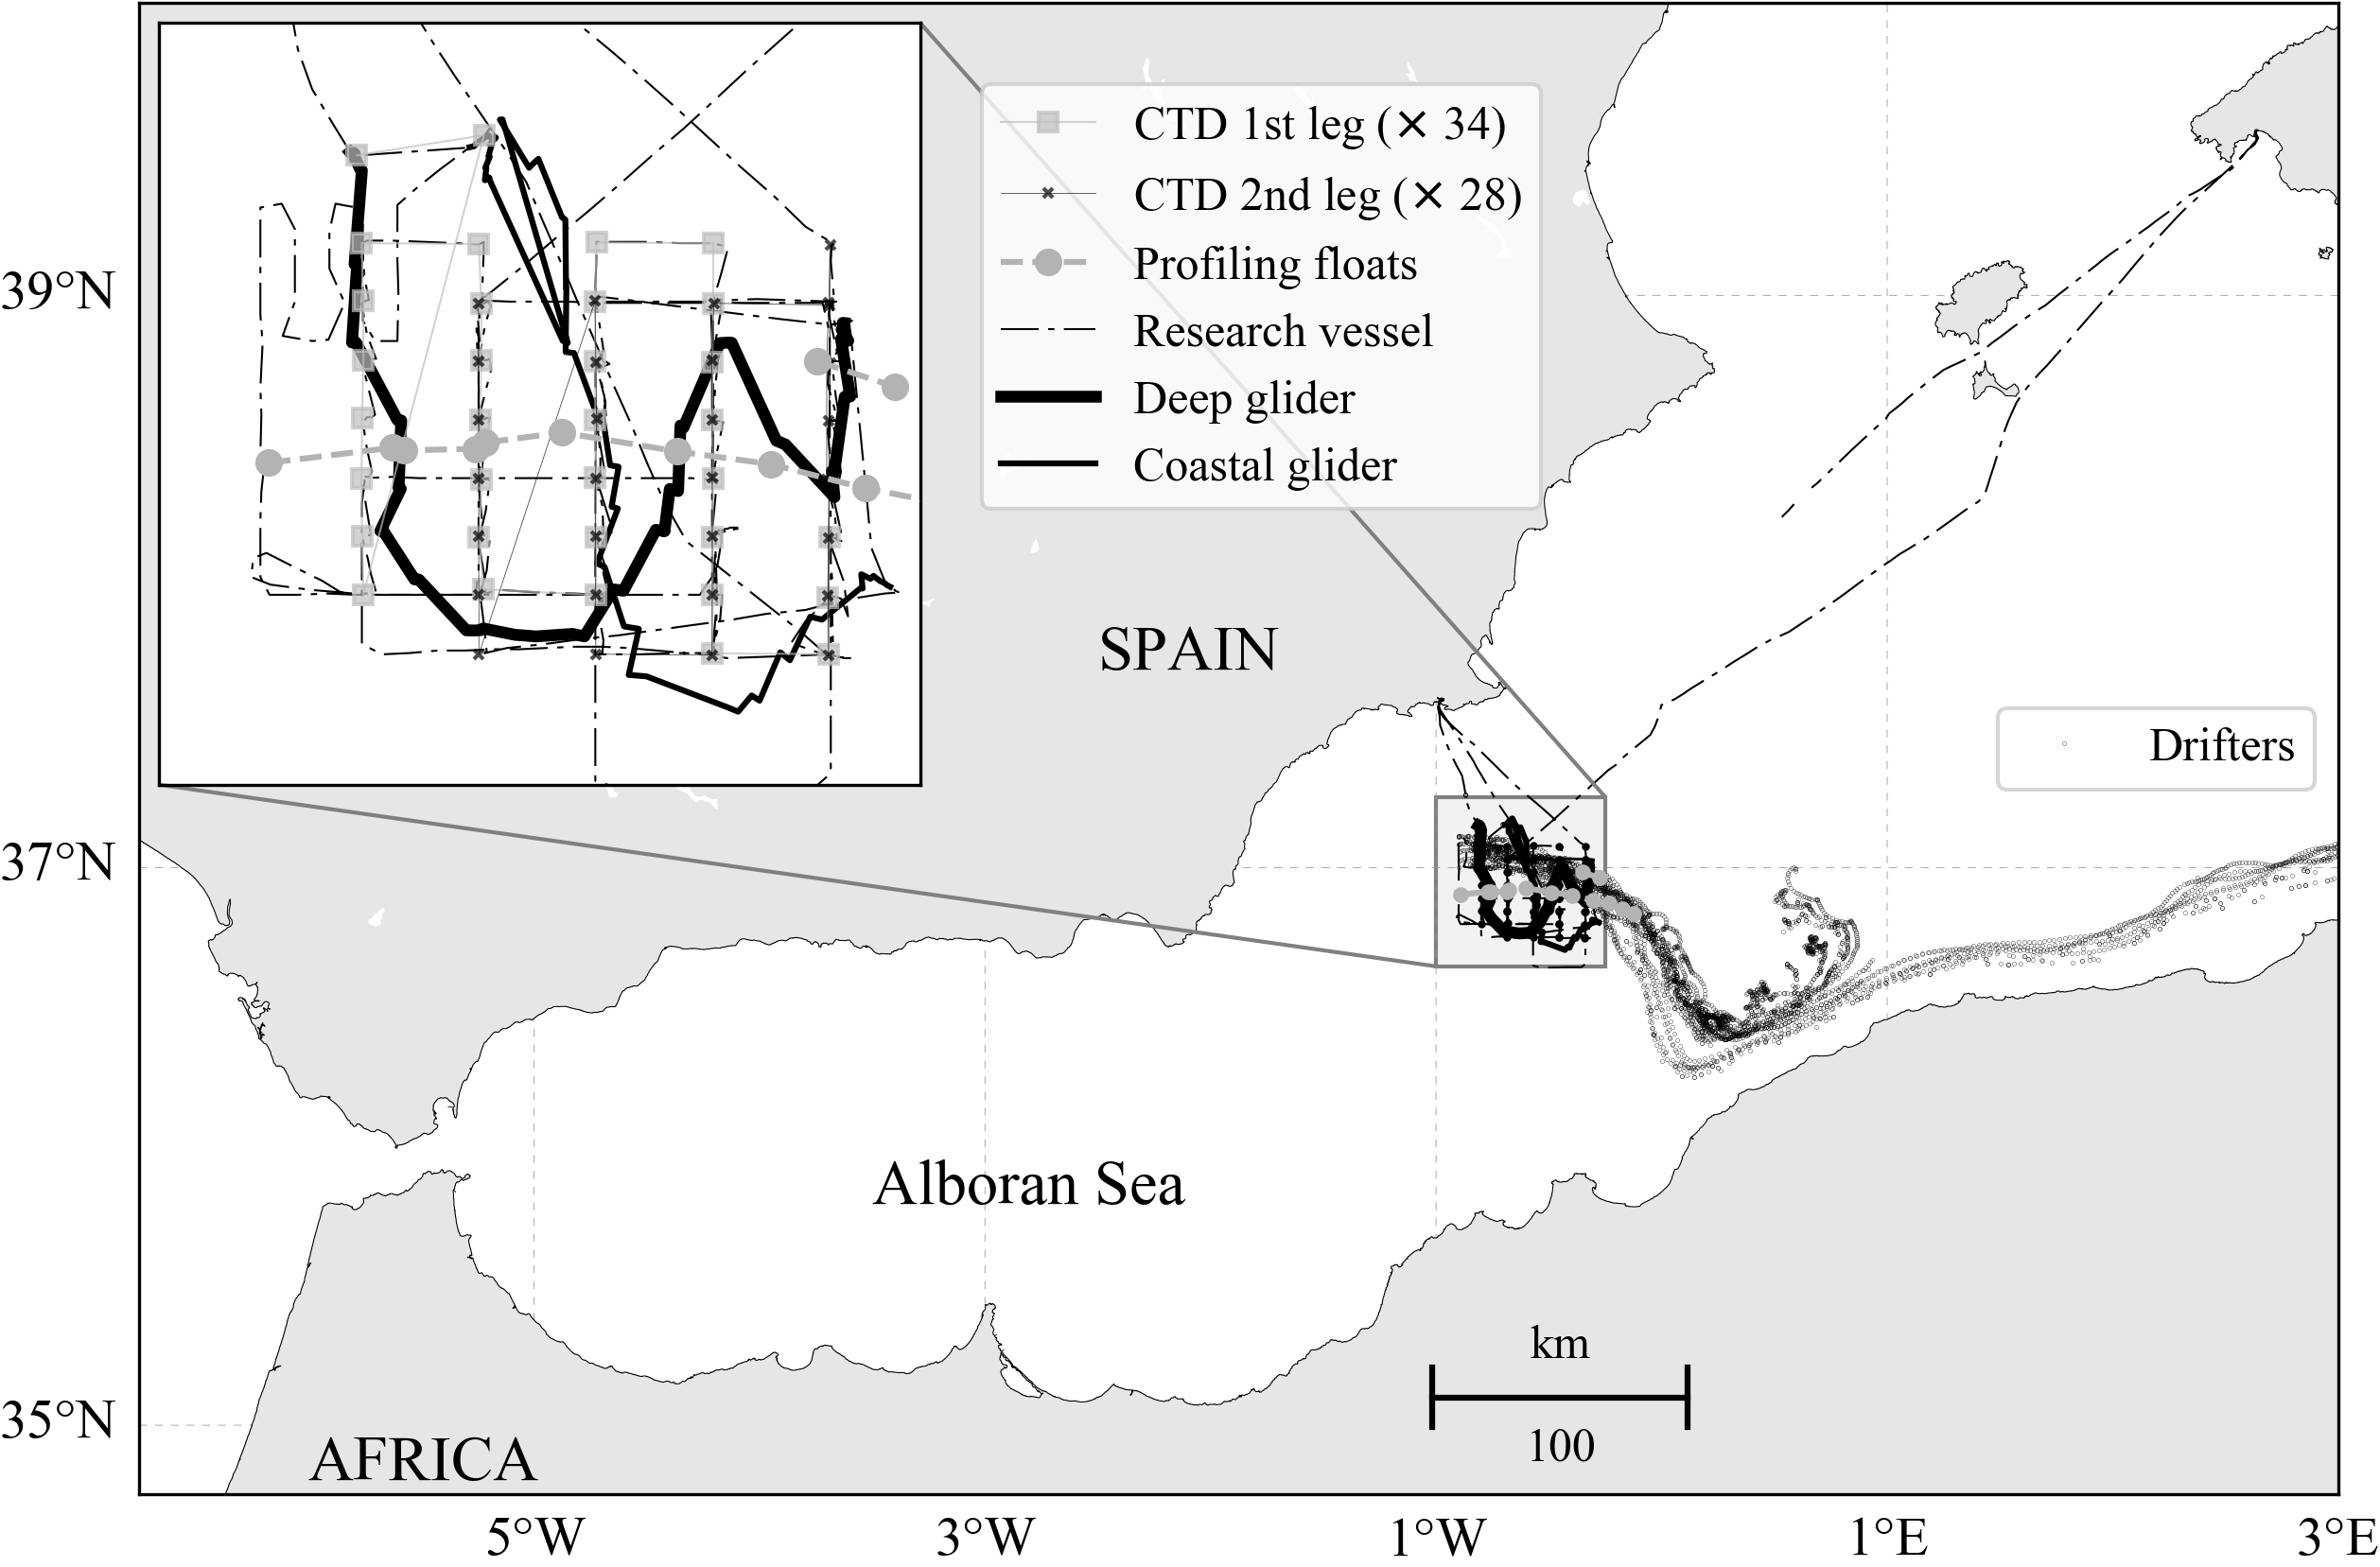
\includegraphics[width=.5\textwidth]{fig01.png}
\caption{Area of study, positions and trajectories of the main platforms. The close-up view on displays the glider and the CTD measurements.\label{fig1:general}}
\end{figure}

\subsection{General oceanographic context}

The definitive sampling area was not firmly decided until a few days before the start of the mission. Prior to the experiment, satellite images of sea surface temperature (SST) and chlorophyll-a concentration were acquired from the Ocean Color Data server (\url{https://oceandata.sci.gsfc.nasa.gov/}, last accessed August 3, 2018) in order to provide an overview of the surface oceanic features apparent in the Alboran Sea. A well-defined front separating Atlantic and Mediterranean waters and exhibiting filament-like structures was selected as the study area (see rectangular boxes in Figs.~\ref{fig1:general} and \ref{fig2:SST}). 

The pair of images indicates that the front position slightly changed between May 25 and 30. An anticyclonic eddy centered around 36$^{\circ}$30'N, 0$^{\circ}$30'W, according to altimetry data (not shown), slowly followed an eastward trajectory in the following days. Other SST images during the period of interest (not shown here) displayed different temperature values near the front, yet the front position remains stable. 

\begin{figure}[t]
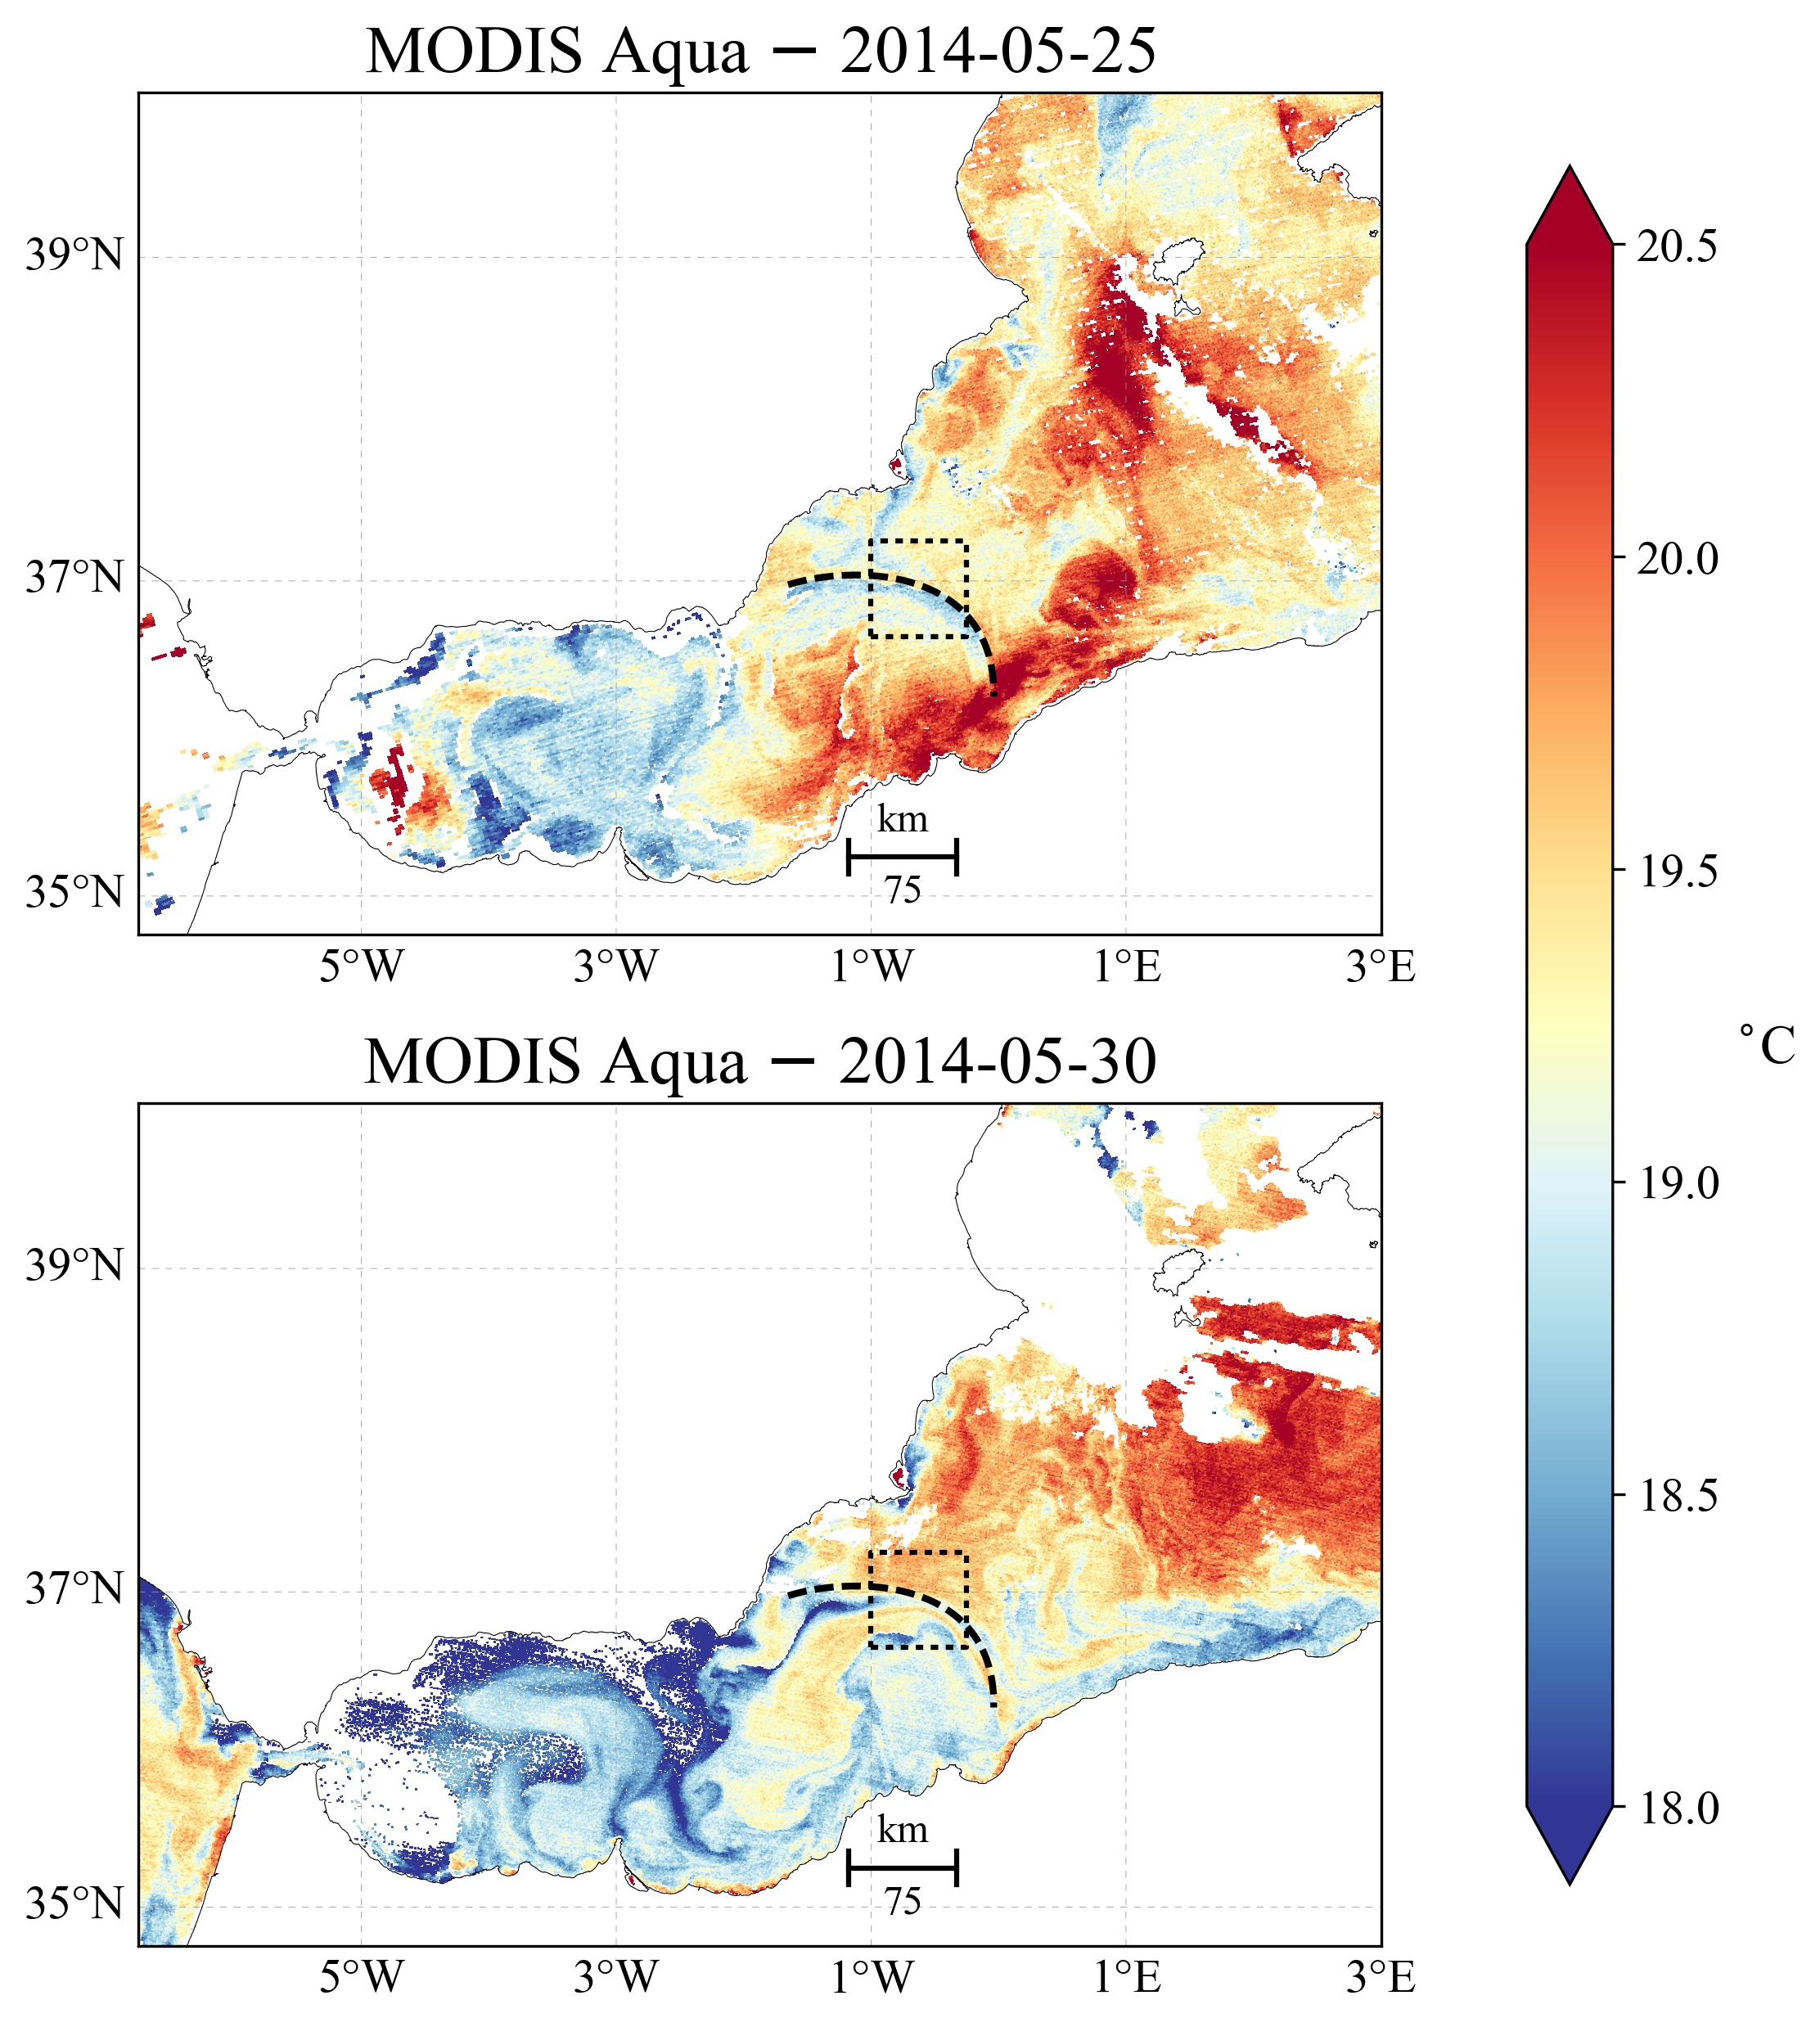
\includegraphics[width=.5\textwidth]{fig02.png}
\caption{Sea surface temperature in the western Mediterranean Sea from MODIS sensor onboard Aqua satellite corresponding to May 25 and 30, 2014. The dashed black line indicates the approximative position of the front based on the temperature gradient for the period 25--30 May. Level-2, 11 $\mu m$, night-time images were selected. Only pixels with a quality flag equal to 1 (good data) were conserved and represented on the map. Note that the same front position is used in the subsequent figures.\label{fig2:SST}}
\end{figure}

\subsection{In situ data}

Whereas the remote sensing measurements helped in the mission design and the front detection, in situ observation were essential to fulfill the mission objectives. The different platforms deployed for the data collection are presented hereinafter.

\subsubsection{Research vessel}

The SOCIB coastal research vessel (R/V) was used to sample the area with vertical profiles acquired though the CTD. Two distinct CTD surveys were performed on a 10~km $\times$ 5~km resolution grid, as depicted in Fig.~\ref{fig3:CTD}: the first survey was run from May 26 to 27 and consisted of 34 casts along 5 meridional legs. The second survey took place from May 29 to 30 and was made up of 28 casts. The casts from both surveys were performed at almost similar locations in order to allow for detecting changes between the two periods. 

\begin{figure}[t]
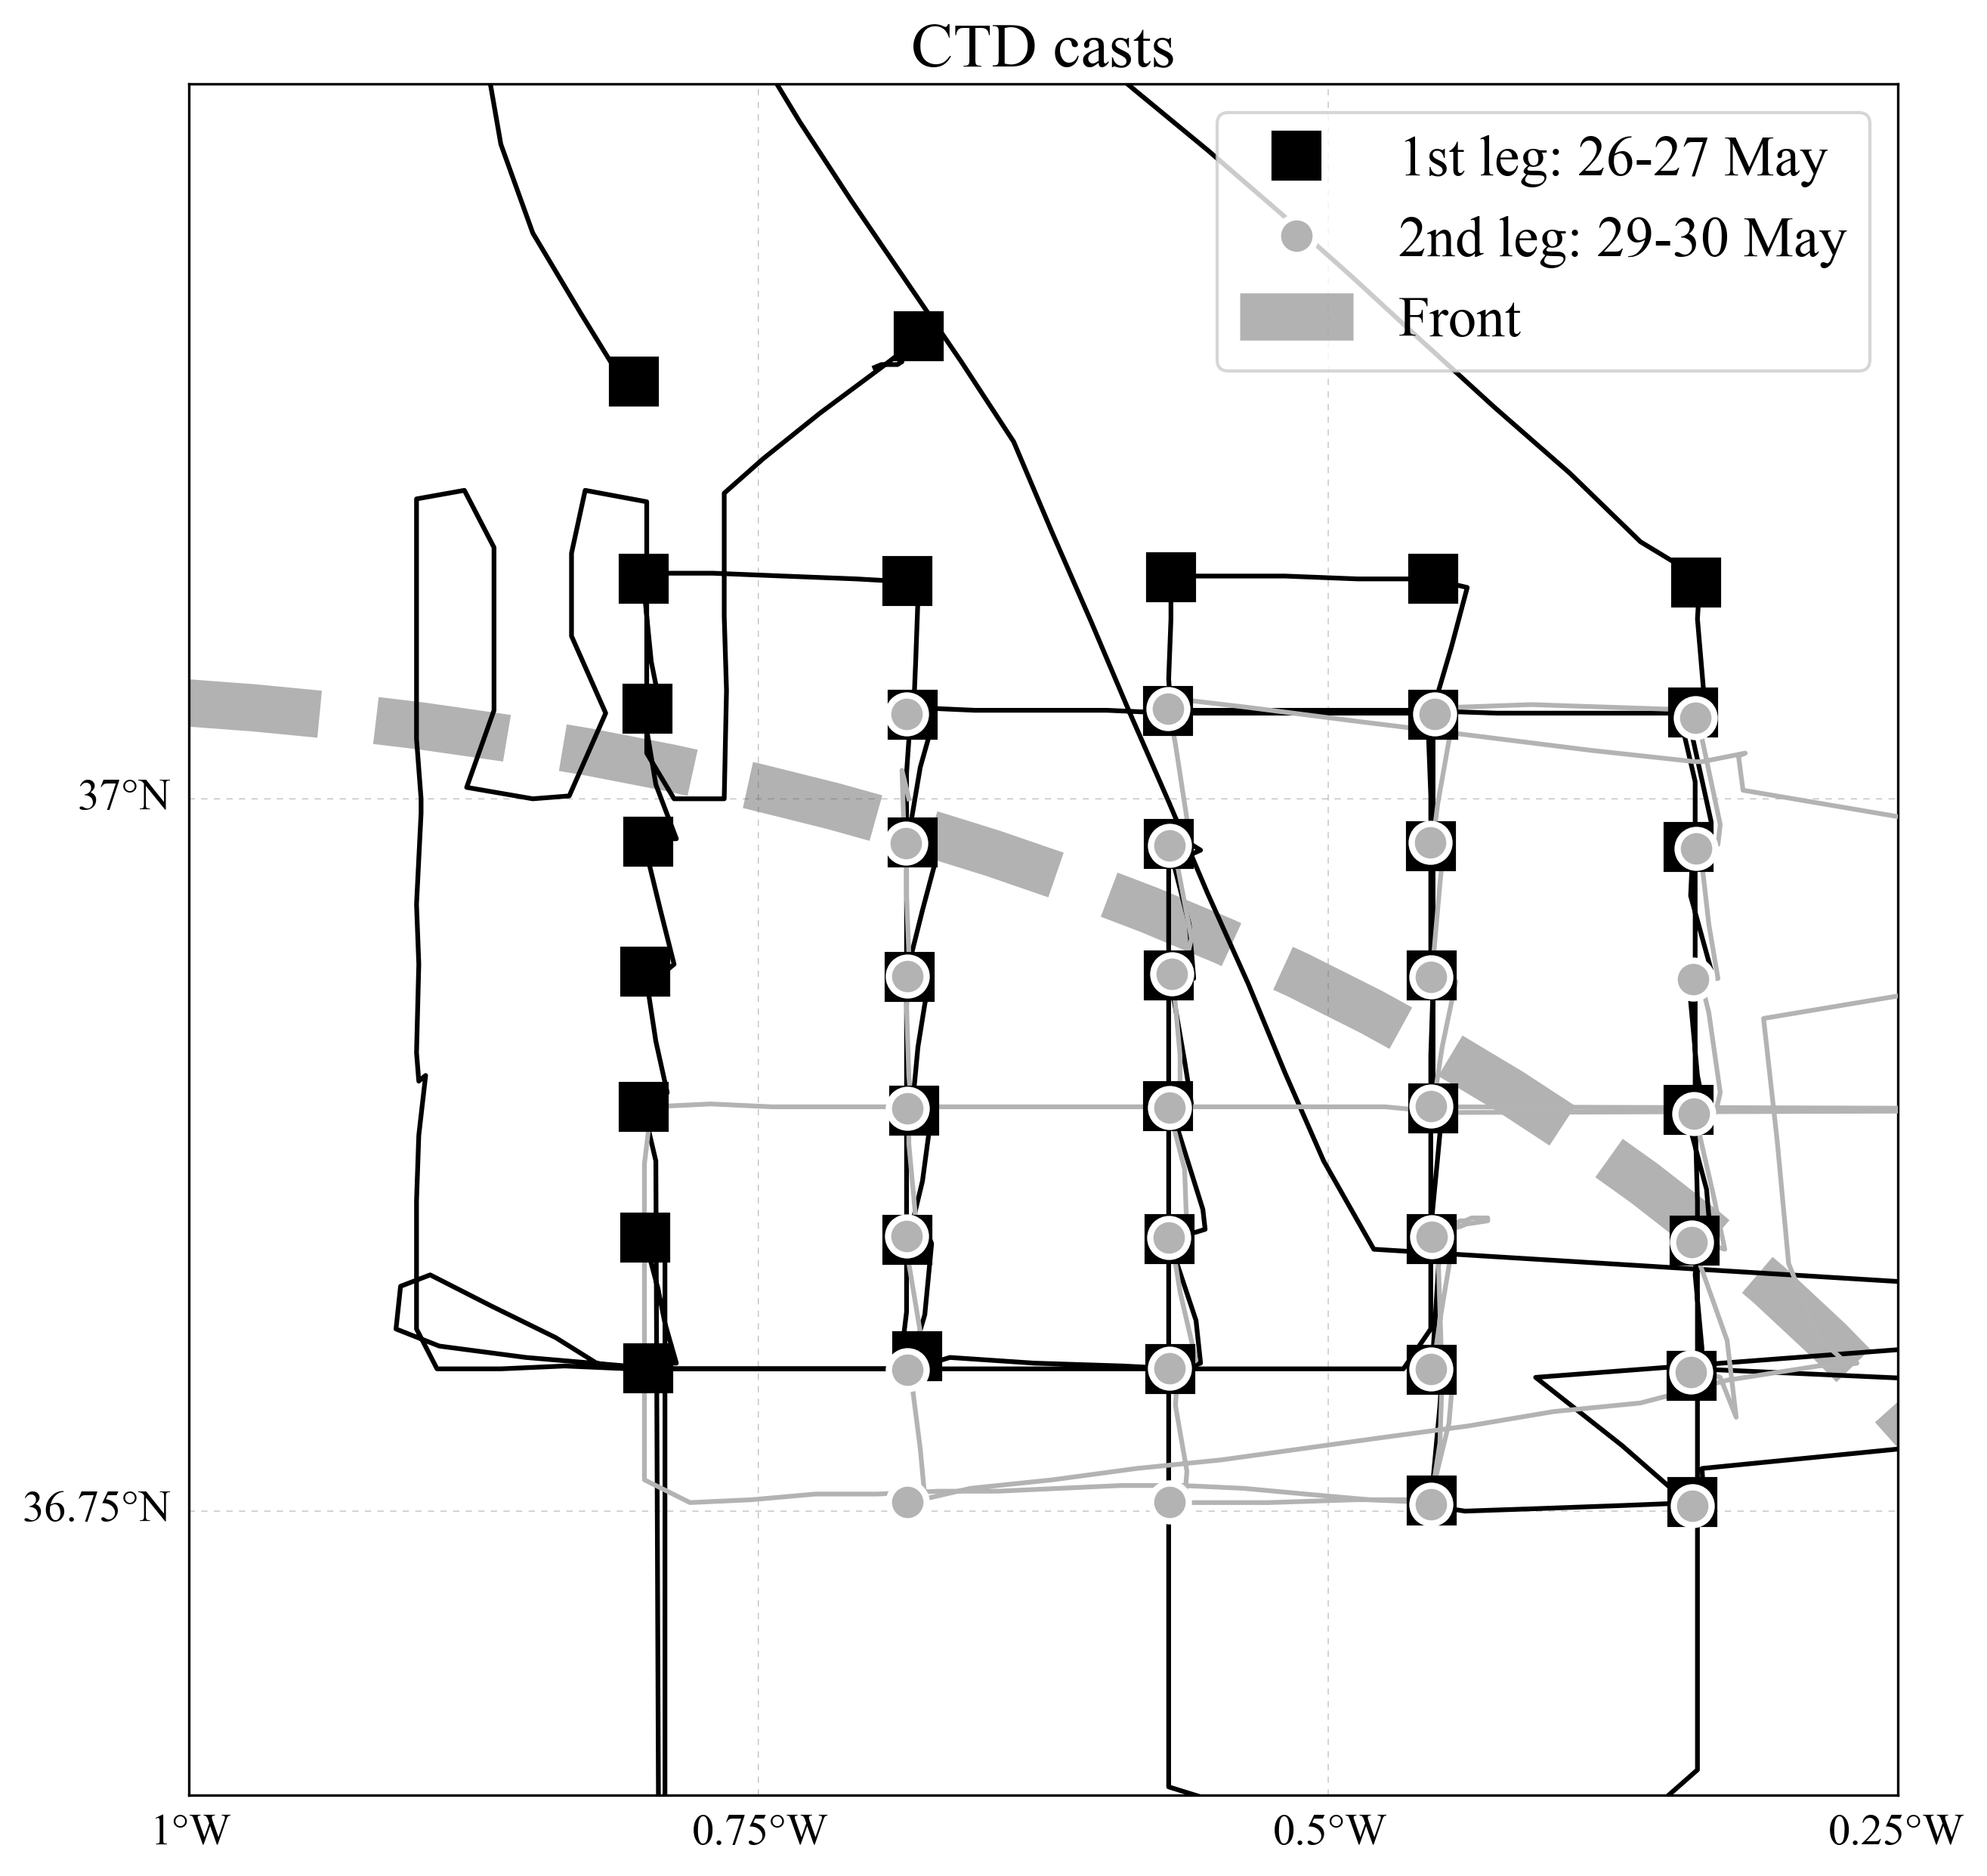
\includegraphics[width=.5\textwidth]{fig03.png}
\caption{The CTD casts were organised in 5 legs that crossed the front and were repeated over 2 periods, at the beginning and the end of the mission.\label{fig3:CTD}.}
\end{figure}

The distinct water properties on both sides of the front are evidenced by the T-S diagrams in Fig.~\ref{fig4:TSdiag}, where the colors represent the fluorescence. The salinity range north of the front is roughly between 38 and 38.5, with the exception of a few measurements, and confirms the nature of the Mediterranean Water mass. The fluorescence maximum appears between 14 and 15$^{\circ}$C. South of the front the salinity range is wider while the temperature values are similar to the north.

\begin{figure*}[t]
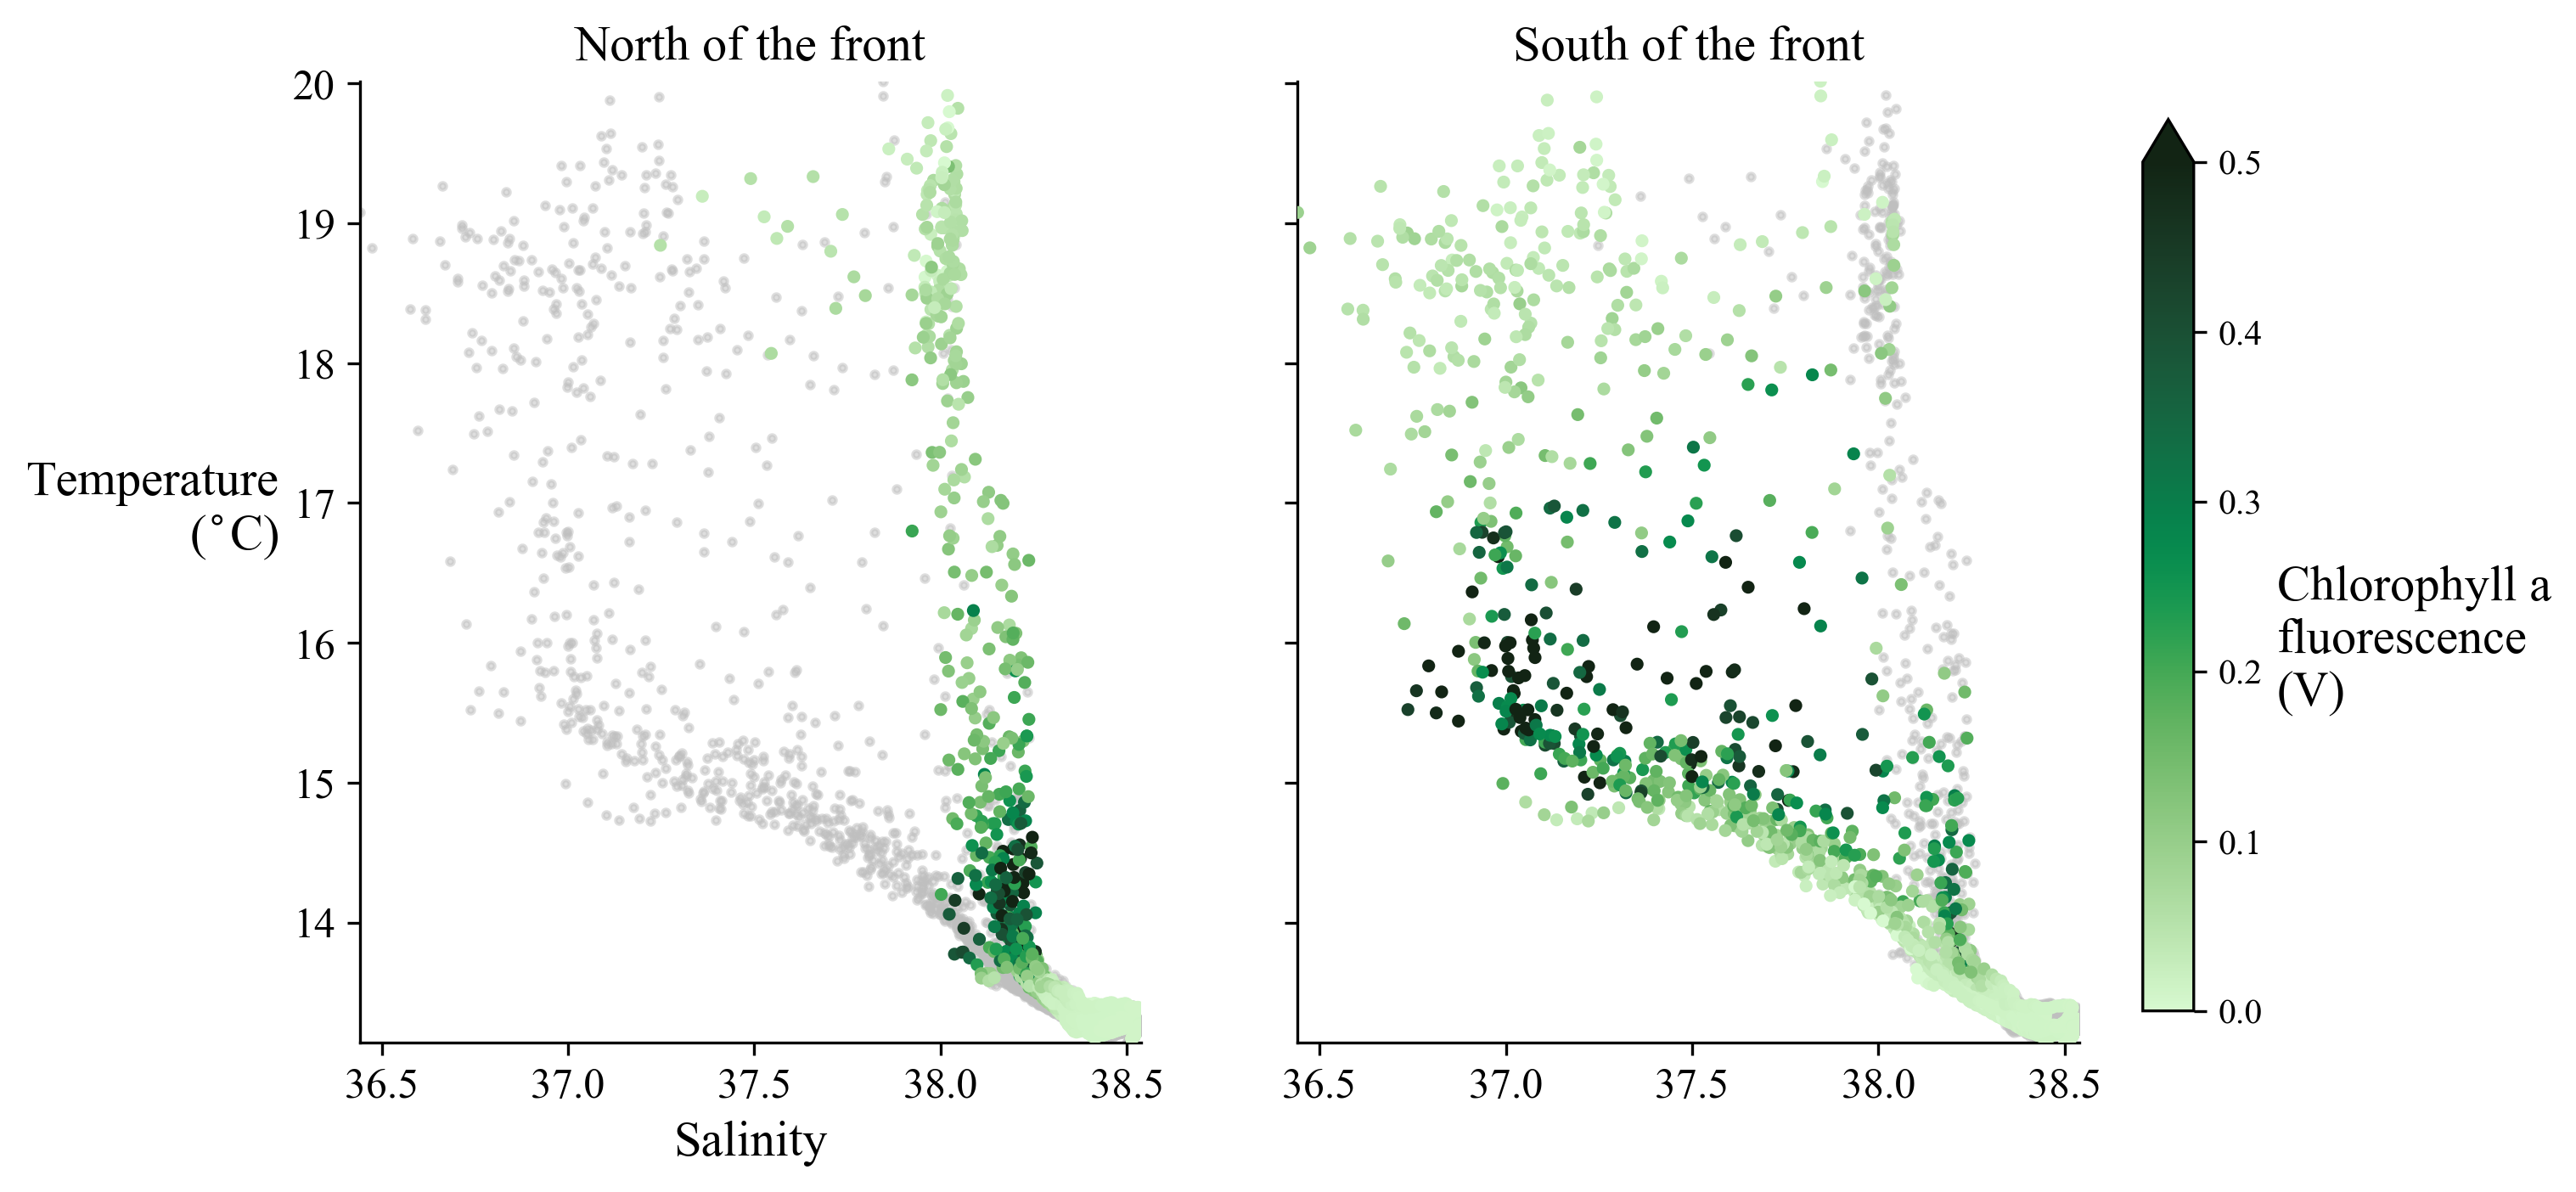
\includegraphics[width=.9\textwidth]{fig04.png}
\caption{The T-S diagrams are shown separately for the casts located north and south of the front (broad, dashed line) \label{fig4:TSdiag}.}
\end{figure*}

In addition to the CTDs, the R/V thermosalinograph continuously acquired temperature and conductivity along the ship track, from which near surface salinity is derived (Fig.~\ref{fig3:thermosal}). The R/V weather station acquired air temperature, pressure, wind speed and direction during the whole duration of the mission. Direct measurements of currents were performed with acoustic Doppler current profiler and are presented in Sec.~\ref{sec:adcp}. 

\begin{figure*}[t]
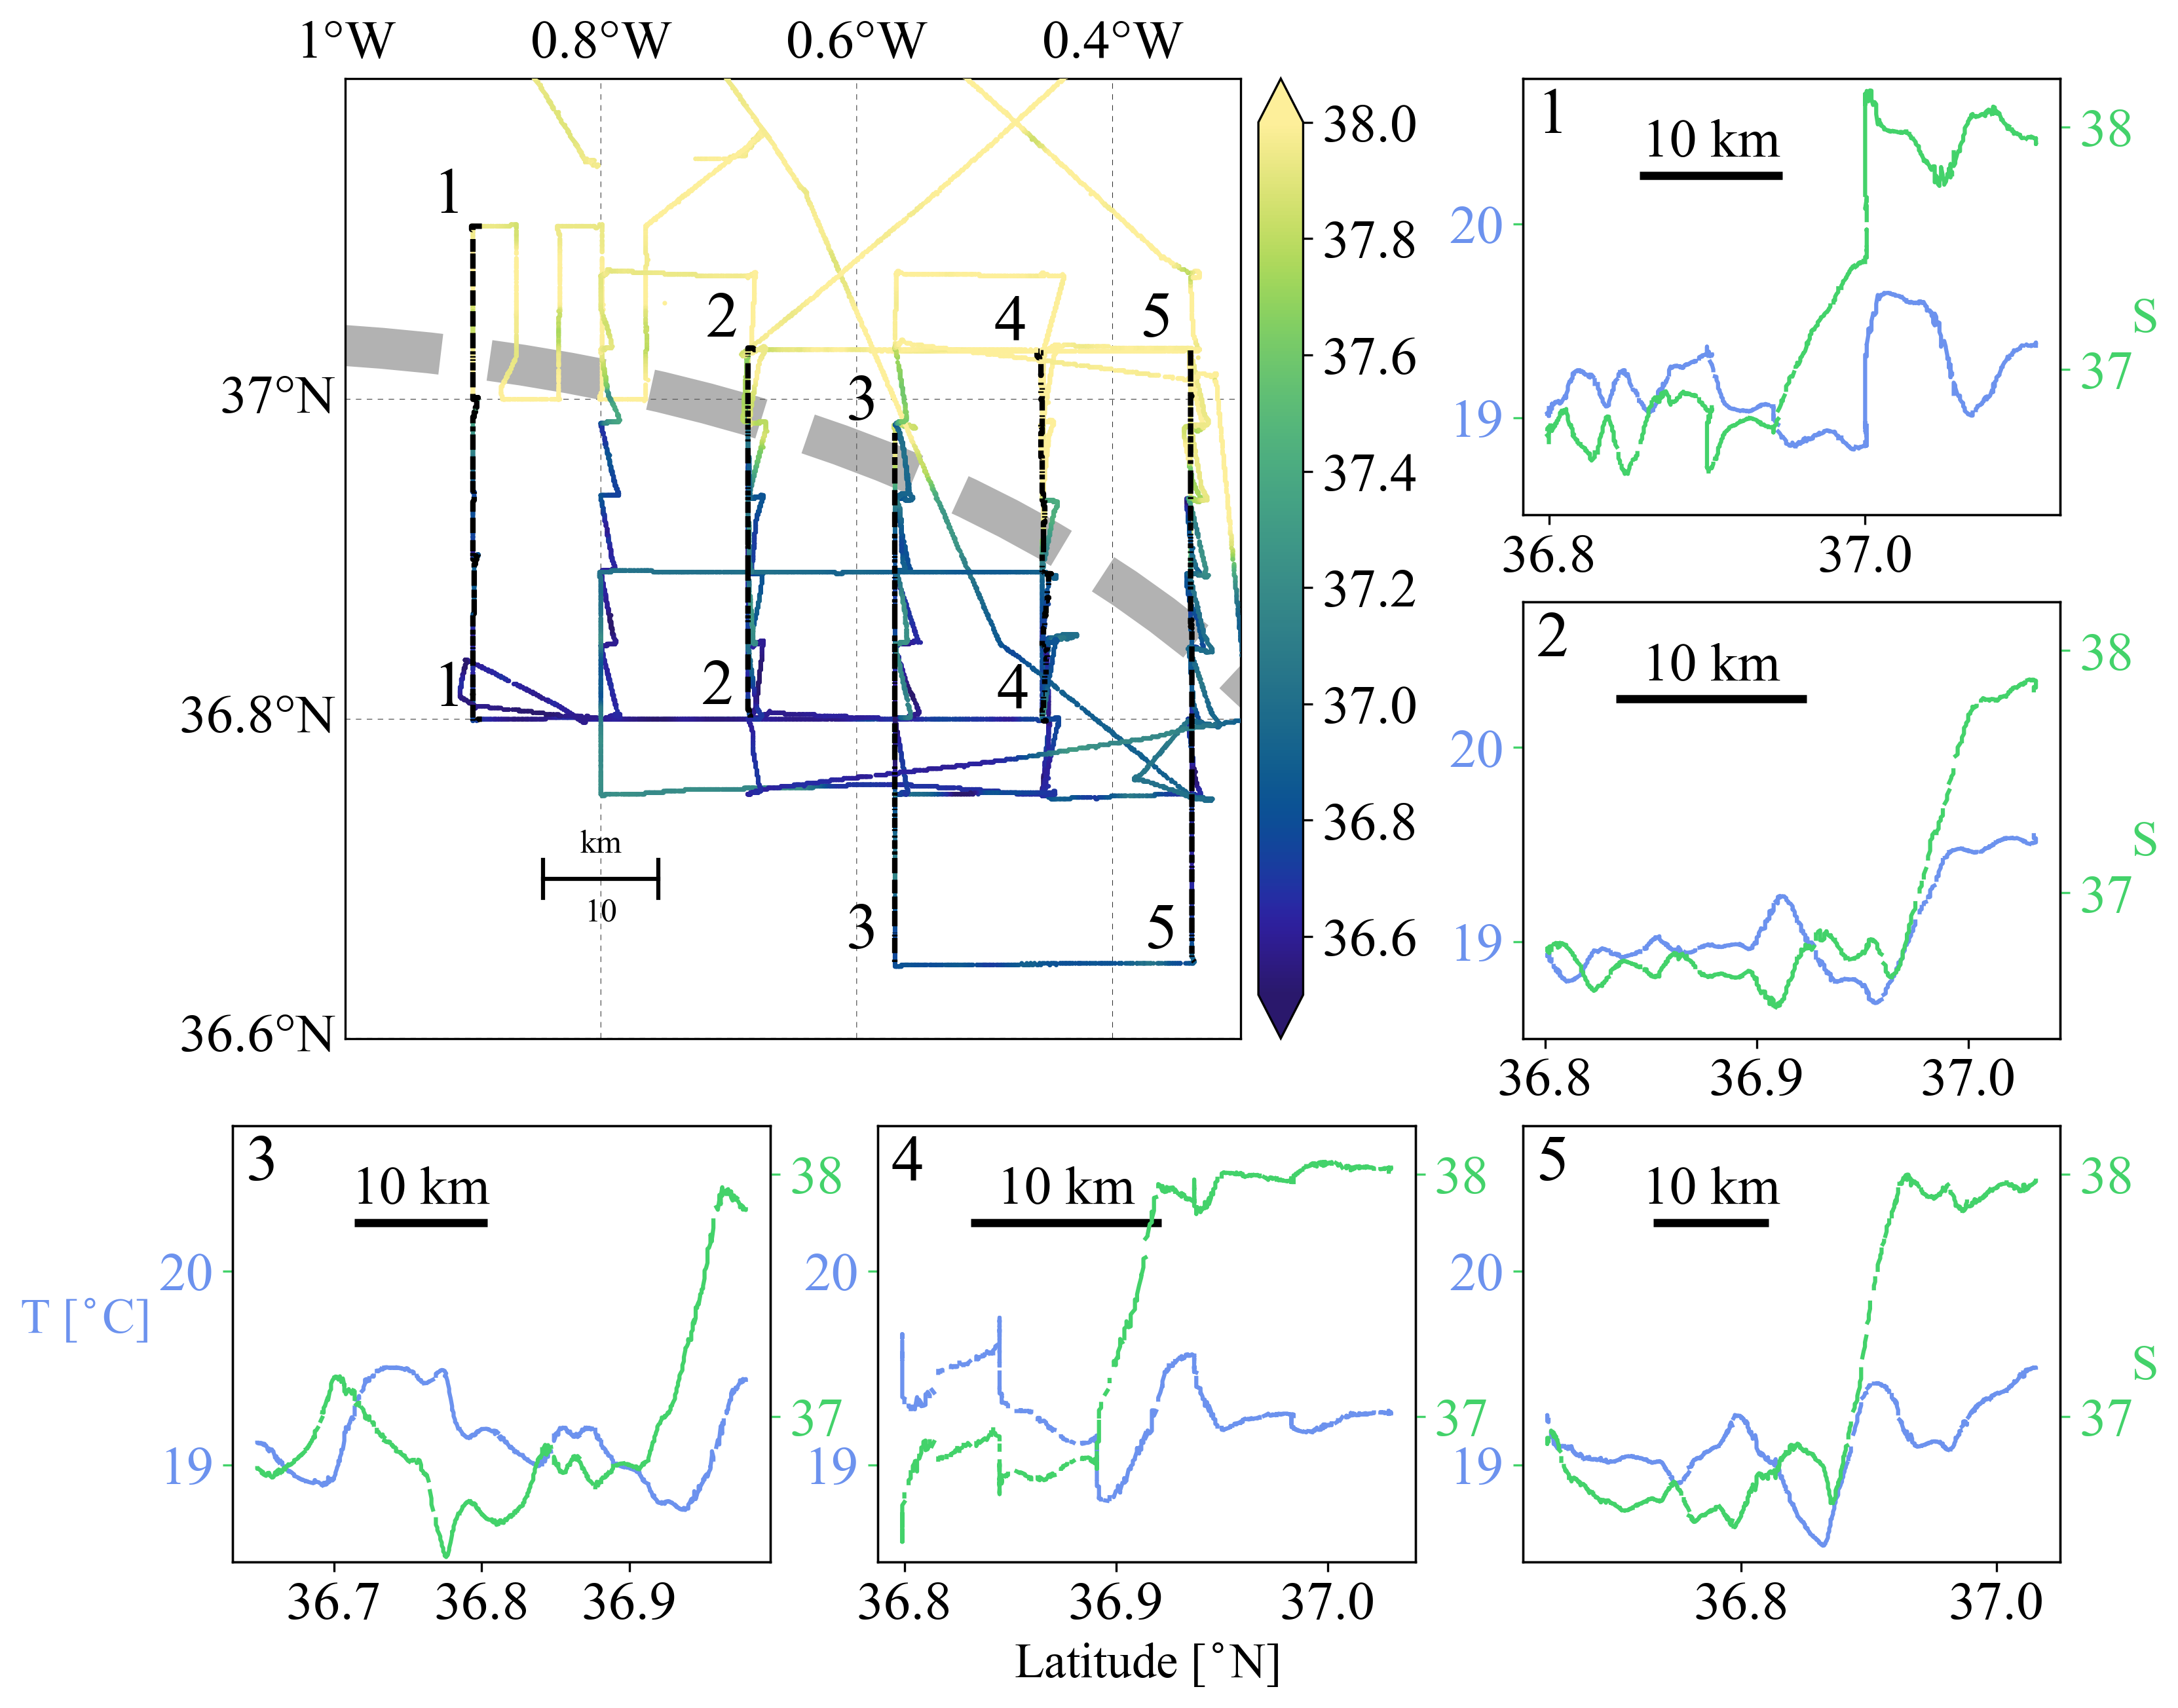
\includegraphics[width=.95\textwidth]{fig05.png}
\caption{The near-surface salinity (colored dots) measured by the thermosalinograph evidences the strong horizontal gradients, in agreement with the front position as obtained using the SST (broad, dashed line). The 5 subplots depict the temperature and salinity along select meridional tracks. \label{fig3:thermosal}}
\end{figure*}

\subsubsection{Gliders}

To collect measurements addressing the submesoscale, two gliders were deployed on May 25 inside the study area. The coastal glider carried out measurements up to 200~m depth and the deep glider up to 500~m. The horizontal resolution was about 0.5~km for the shallow and 1~km for the deep glider. The initial sampling strategy consisted in two 50-km long, meridional tracks, 10 kilometers away one from the other, and to repeat these tracks up to 4 times during the experiment. However, due to the strong zonal currents in the frontal zone, different tracks (Fig.~\ref{fig6:glidertracks}) crossing the front several times were made instead.

\begin{figure}[t]
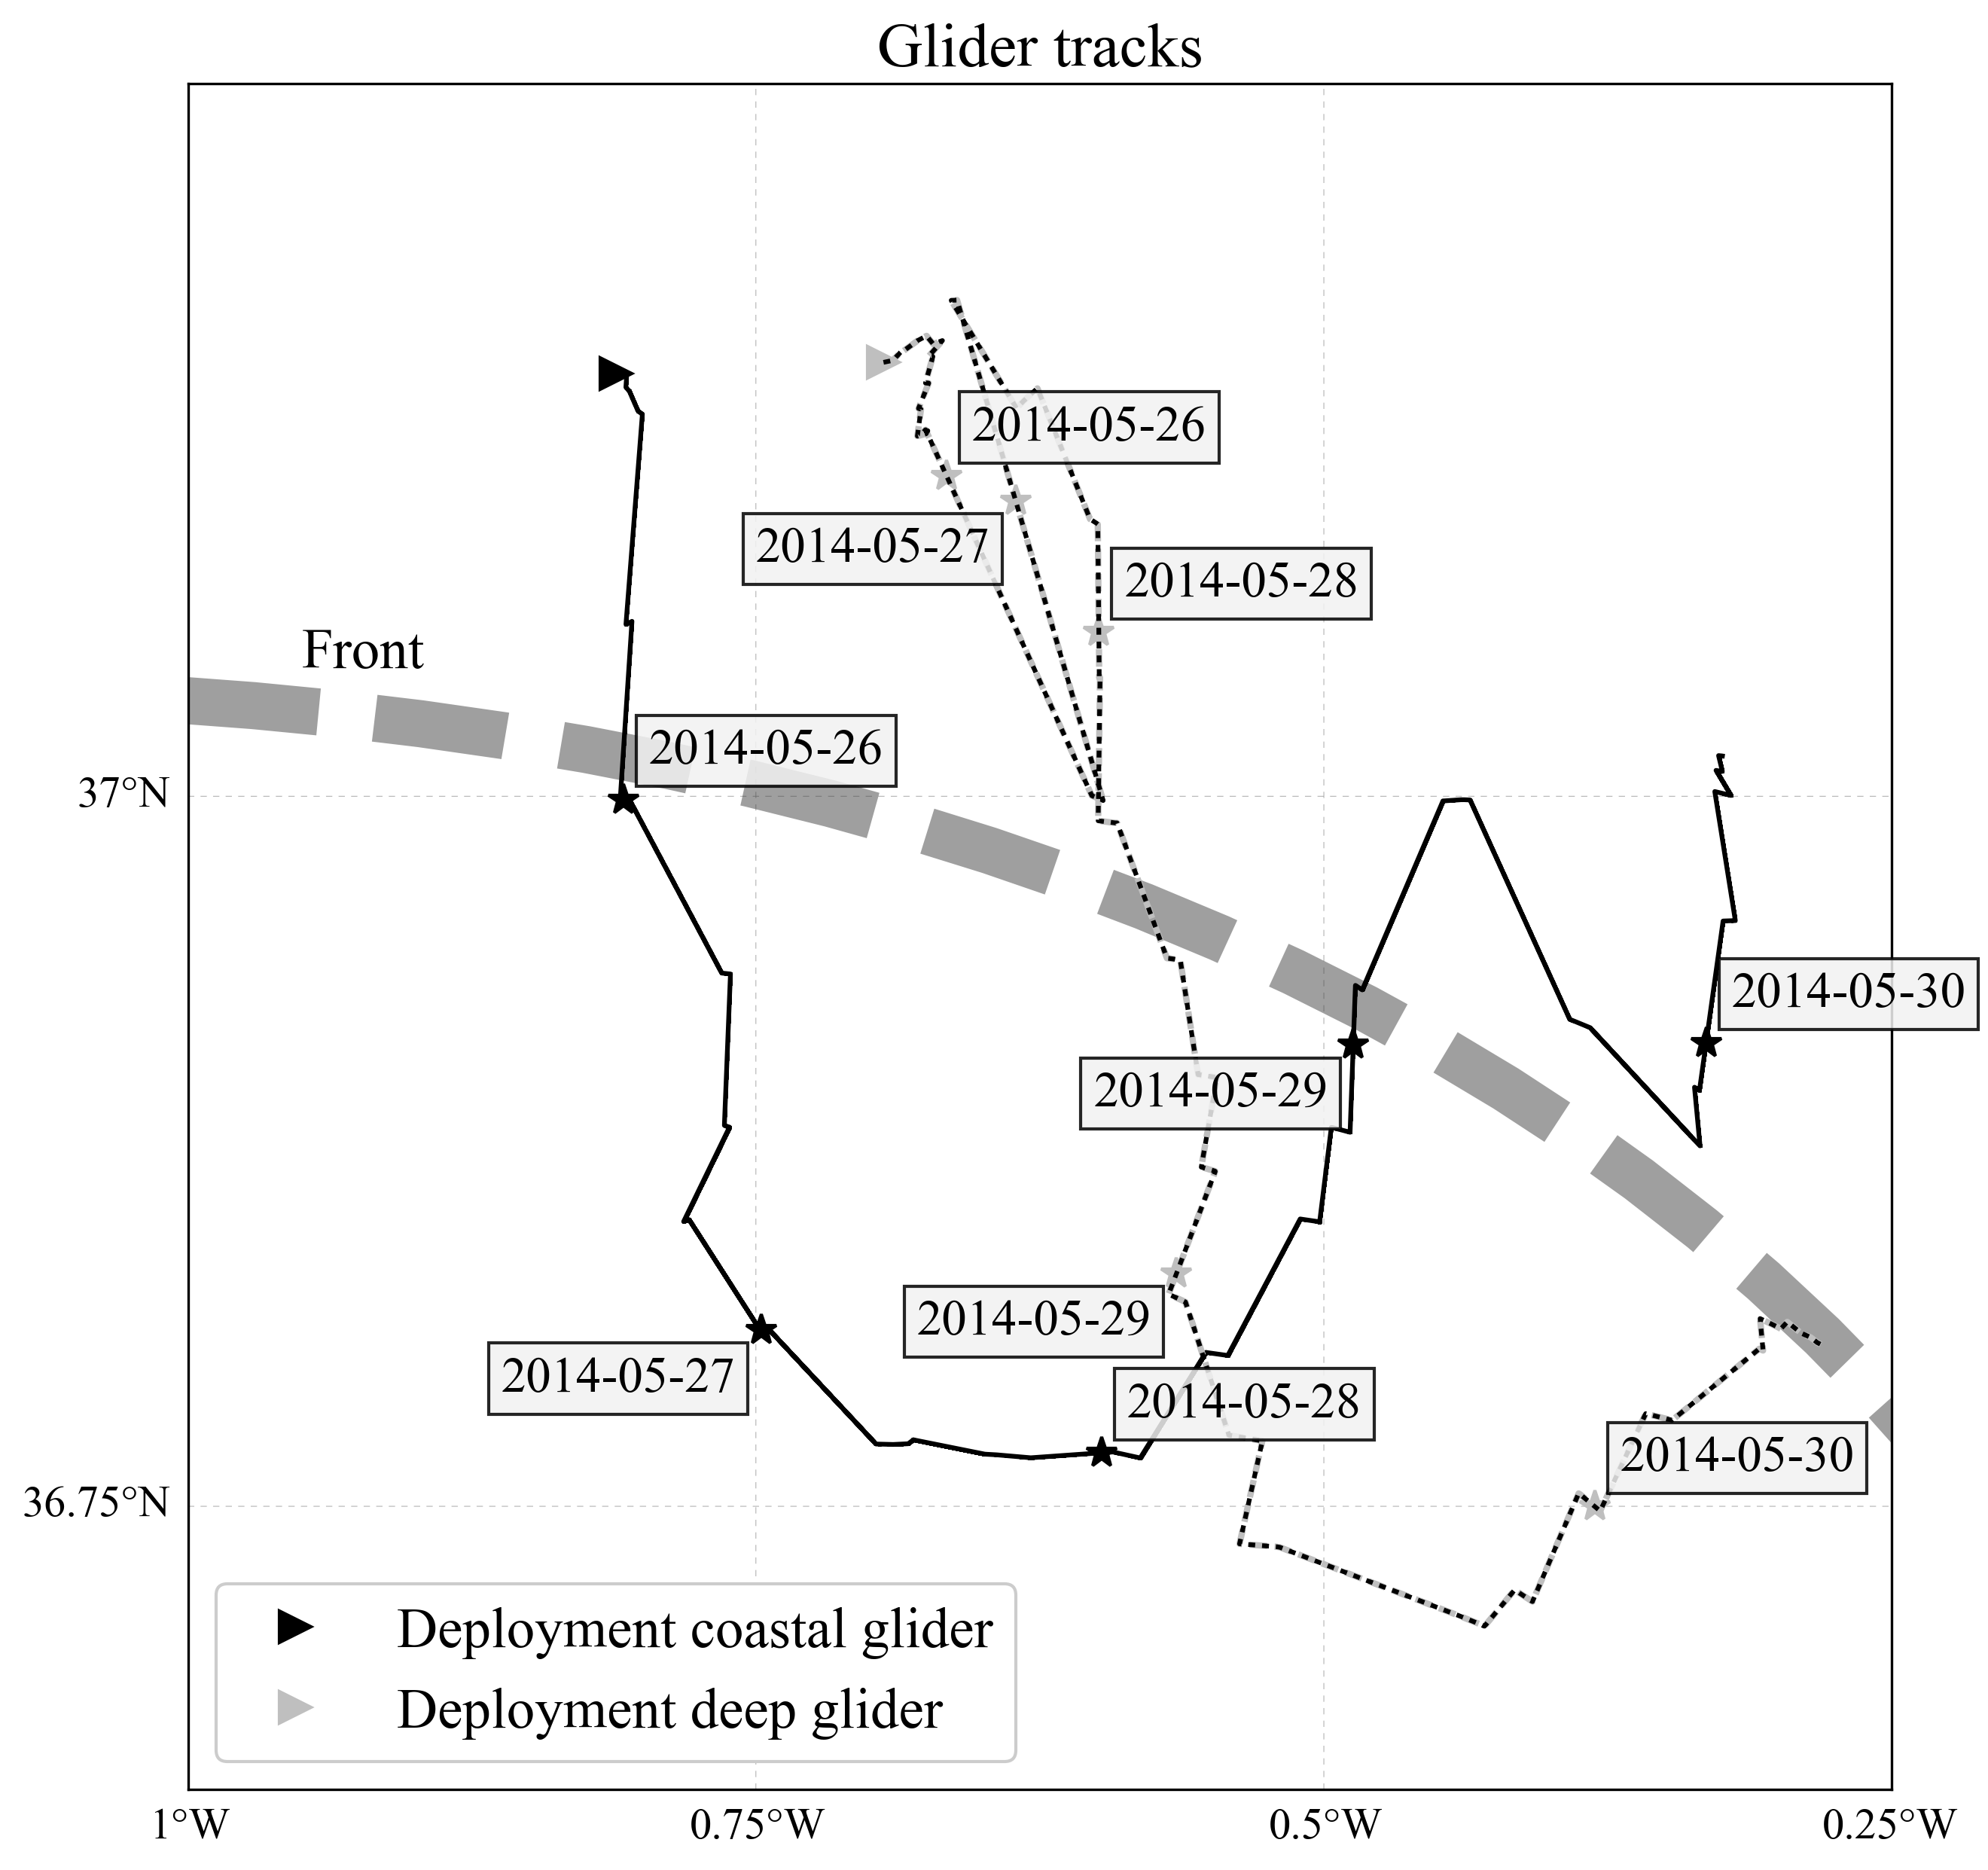
\includegraphics[width=.5\textwidth]{fig06a.png}
\caption{Deployment positions and trajectories of the gliders. Different time instances separated by one day are indicated on the tracks to provide a temporal dimension.\label{fig6:glidertracks}}
\end{figure}

The total number of valid measurements (i.e., discarding the bad and missing values) acquired are 121513 for the deep glider and 226717 for the coastal. The mean vertical separation between 2 consecutive measurements is around 16~cm. Figure~\ref{fig6:glidersections} displays the temperature and salinity sections obtained with the 2 devices. The high density of measurements makes it possible to distinguish small-scale features on both sides of the front, such as strong lateral gradients, subduction or filament structures.  

\begin{figure*}[t]
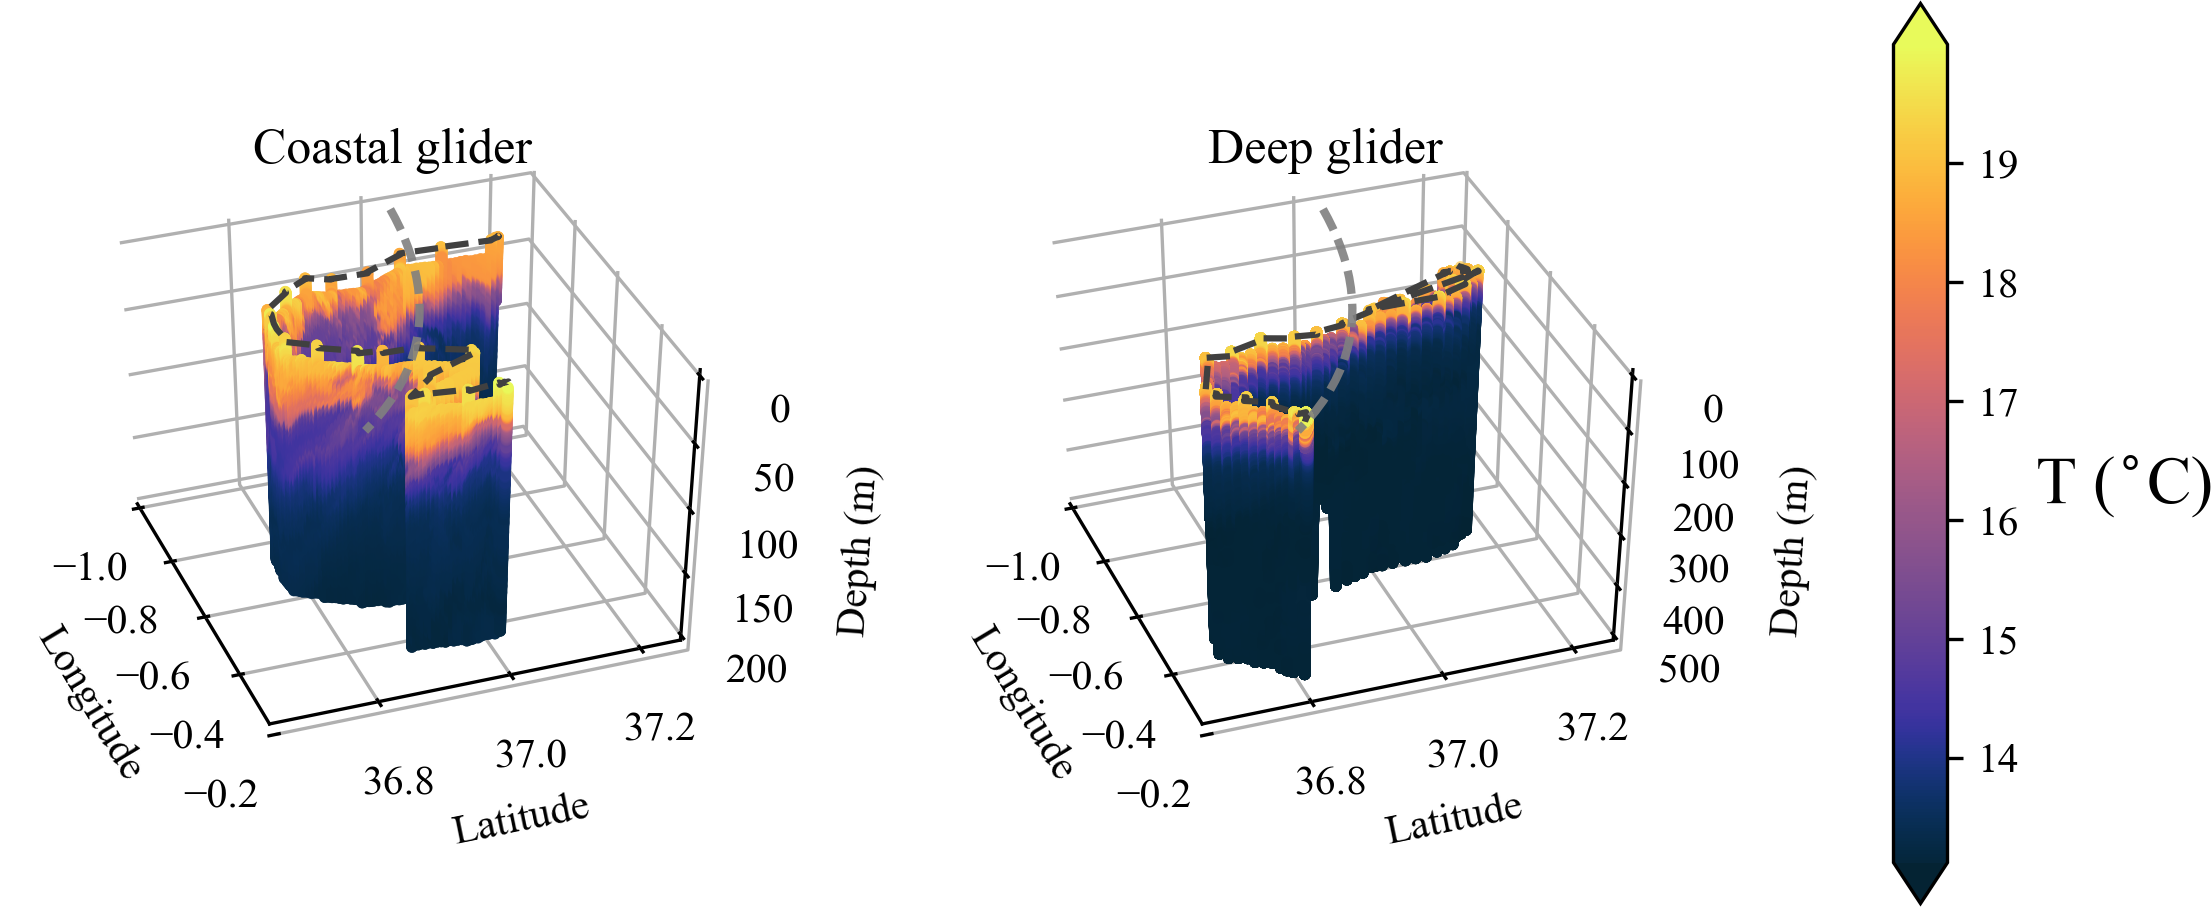
\includegraphics[width=\textwidth]{fig06b.png}\\
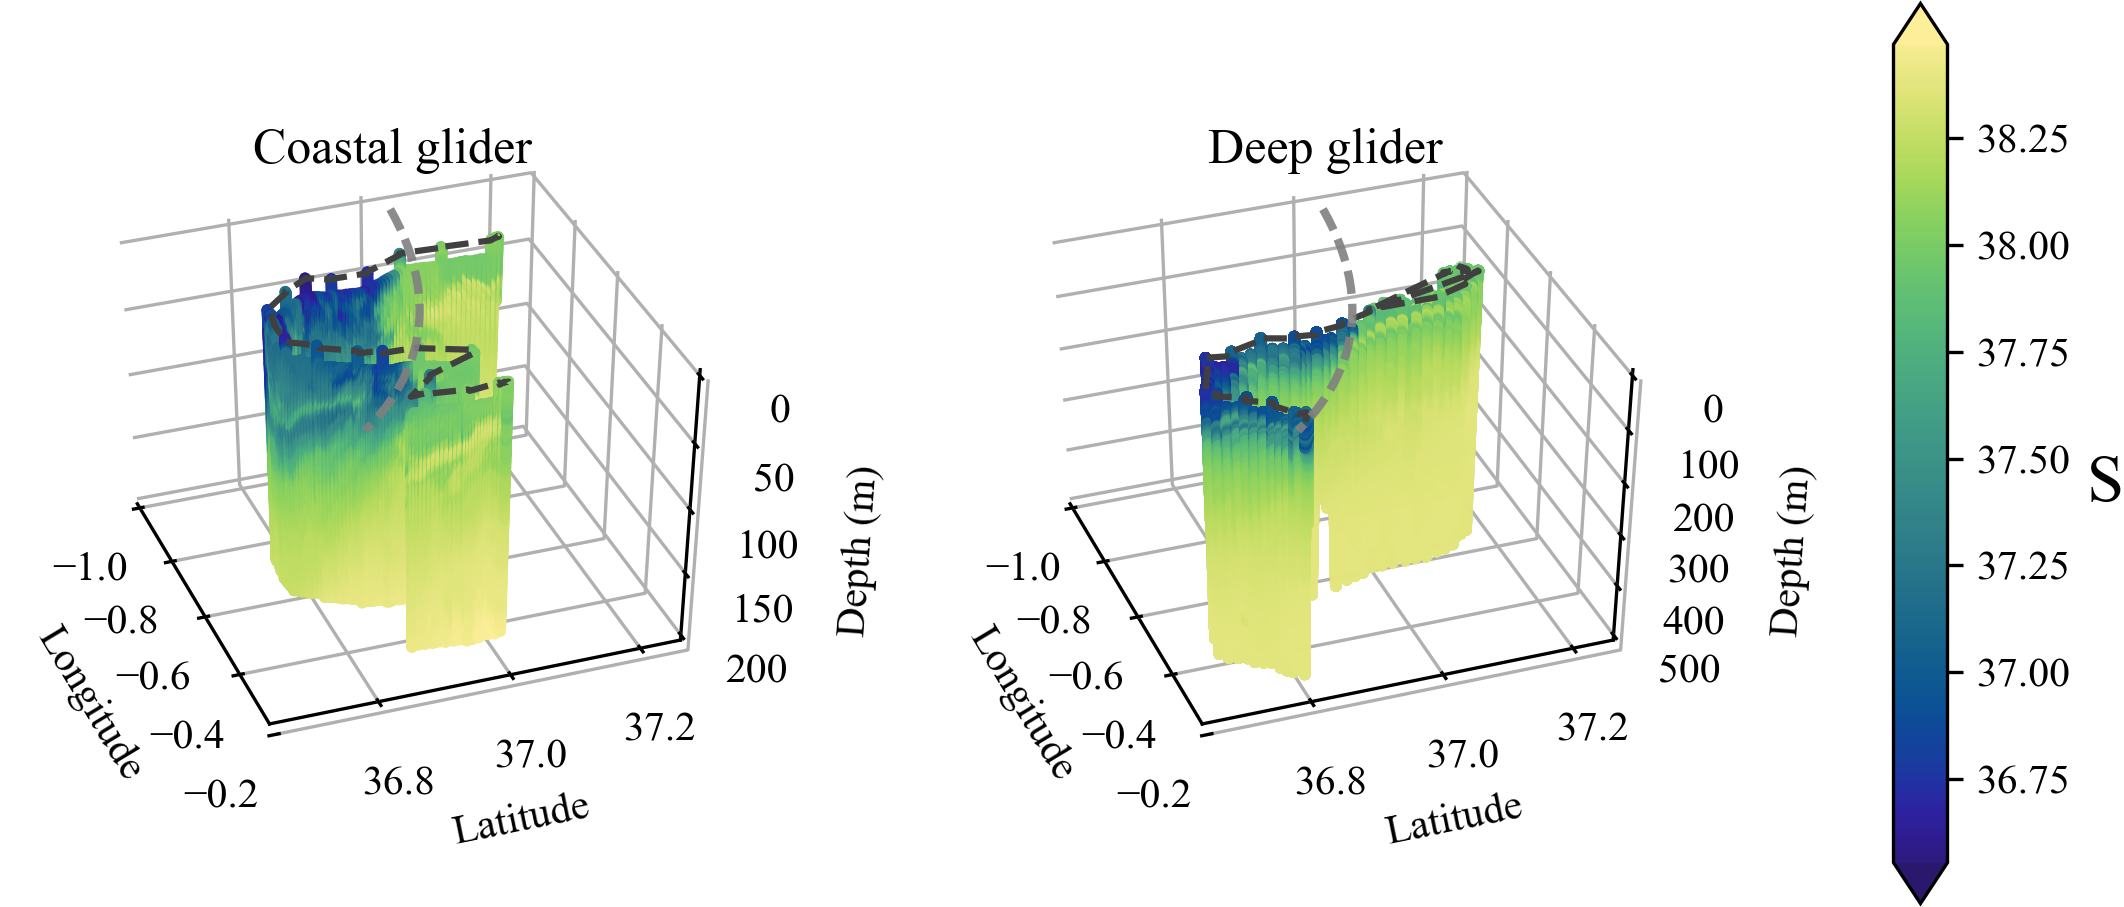
\includegraphics[width=\textwidth]{fig06c.png}
\caption{Temperature and salinity measured by the two gliders. The front position is shown as a dashed, grey line.\label{fig6:glidersections}}
\end{figure*}

The gliders follow a 3-dimensional trajectory in the water column but for some specific usages it is sometimes more convenient to have the glider data as if they were a series vertical profiles. To do so, a spatial interpolation is applied on the original data, leading to the so-called Level-2 data, further described in Sec.~\ref{sec:processing}.


\subsubsection{Surface drifters}

On May 25, 25 Surface Velocity Program (SVP) drifters were deployed in the frontal area in a tight square pattern with a mean distance between neighbor drifters around 3~km. In the Mediterranean Sea, they have been shown to provide information on the surface dynamics, ranging from basin scales to mesoscale features or coastal currents \citep{POULAIN13}. Almost all the drifters were equipped with a thermistor on the lower part of the buoy to measure sea water temperature. 

11 out the 25 drifters, especially those deployed more to the south, were captured by the intense Algerian Current and followed a trajectory along the coast until a longitude about 5$^{\circ}$30'E. The other drifters were deflected northward about 0$^{\circ}$30'E, then veered northwestward or eastward 
and described cyclonic and anticyclonic trajectories, respectively. Interestingly, all the drifters exhibit a trajectory close to the front position deduced from the SST images, until they encounter the Algerian Current (Fig.~\ref{fig3:drifters}). 

On average the temporal sampling resolution is close to one hour, except for 2 drifters for which the intervals are 4 and 5 hours. The velocities are directly computed from the successive positions and highlight the strength of the Algerian Current with velocities on the order of 1~m/s (Fig.~\ref{fig7:drifterszoom}).    

\begin{figure}[t]
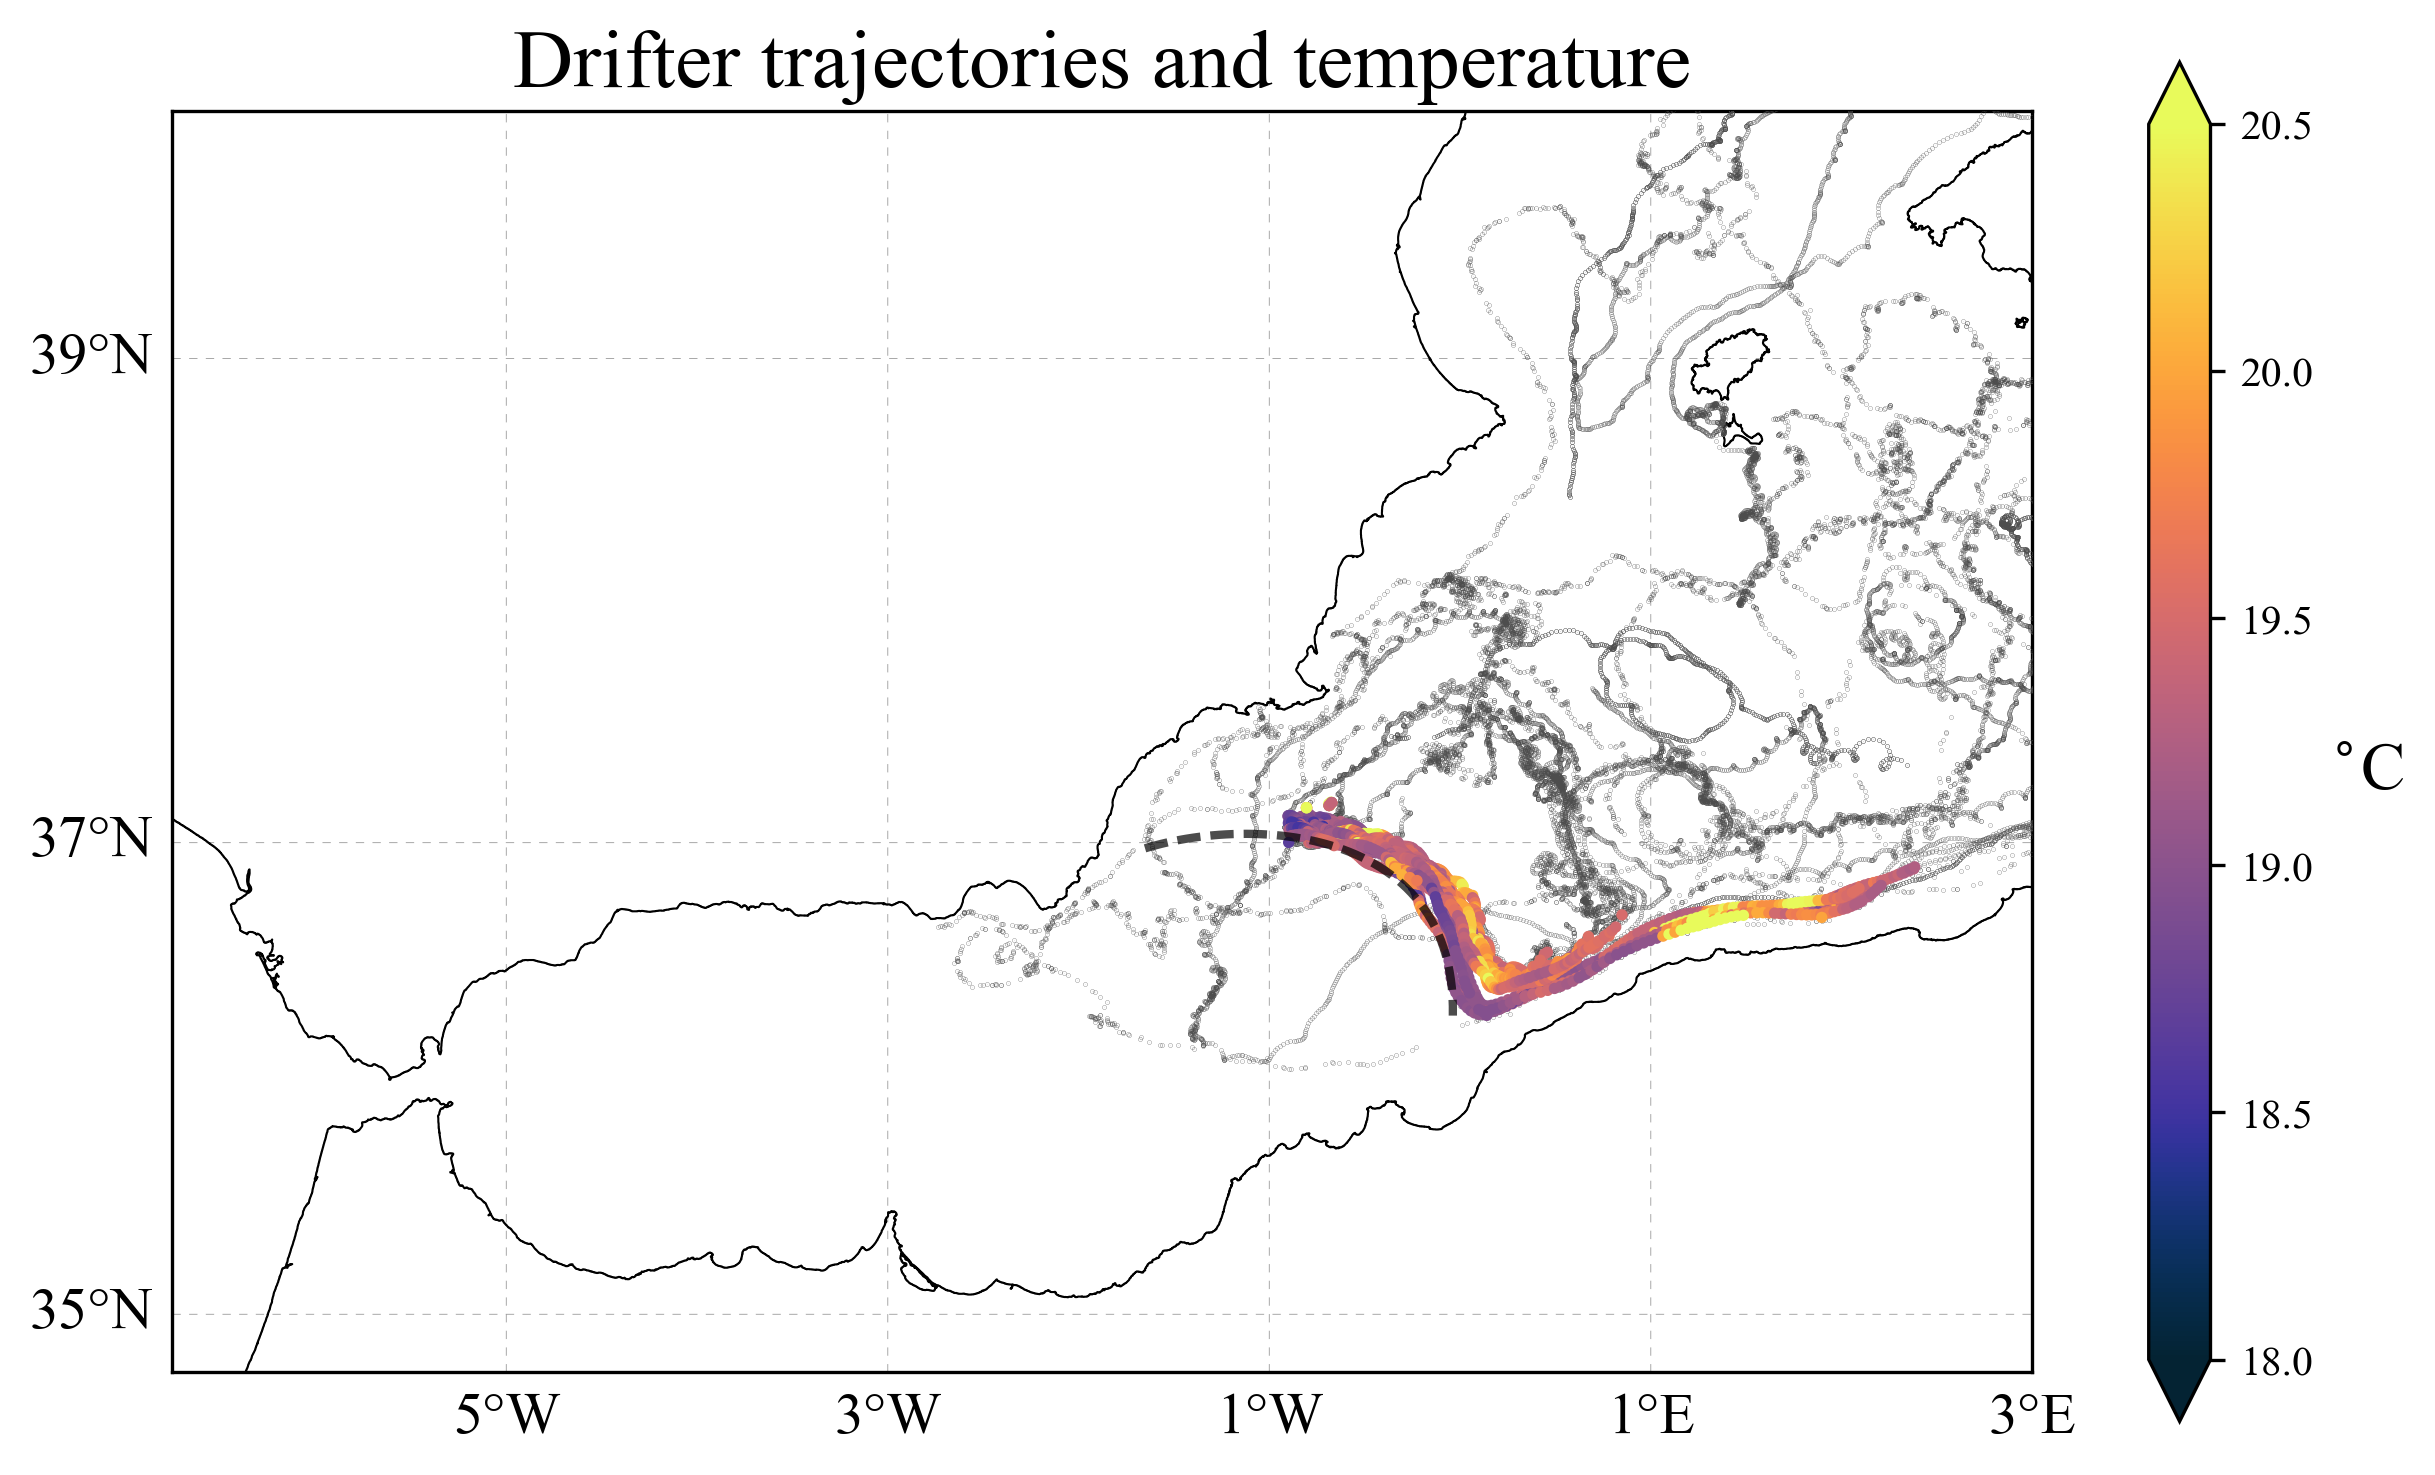
\includegraphics[width=.5\textwidth]{fig07a.png}
\caption{Surface drifter trajectories. For the sake of simplicity and clarity, the temperature, when available, is only shown for the duration of the mission.\label{fig3:drifters}}
\end{figure}

\begin{figure*}[h]
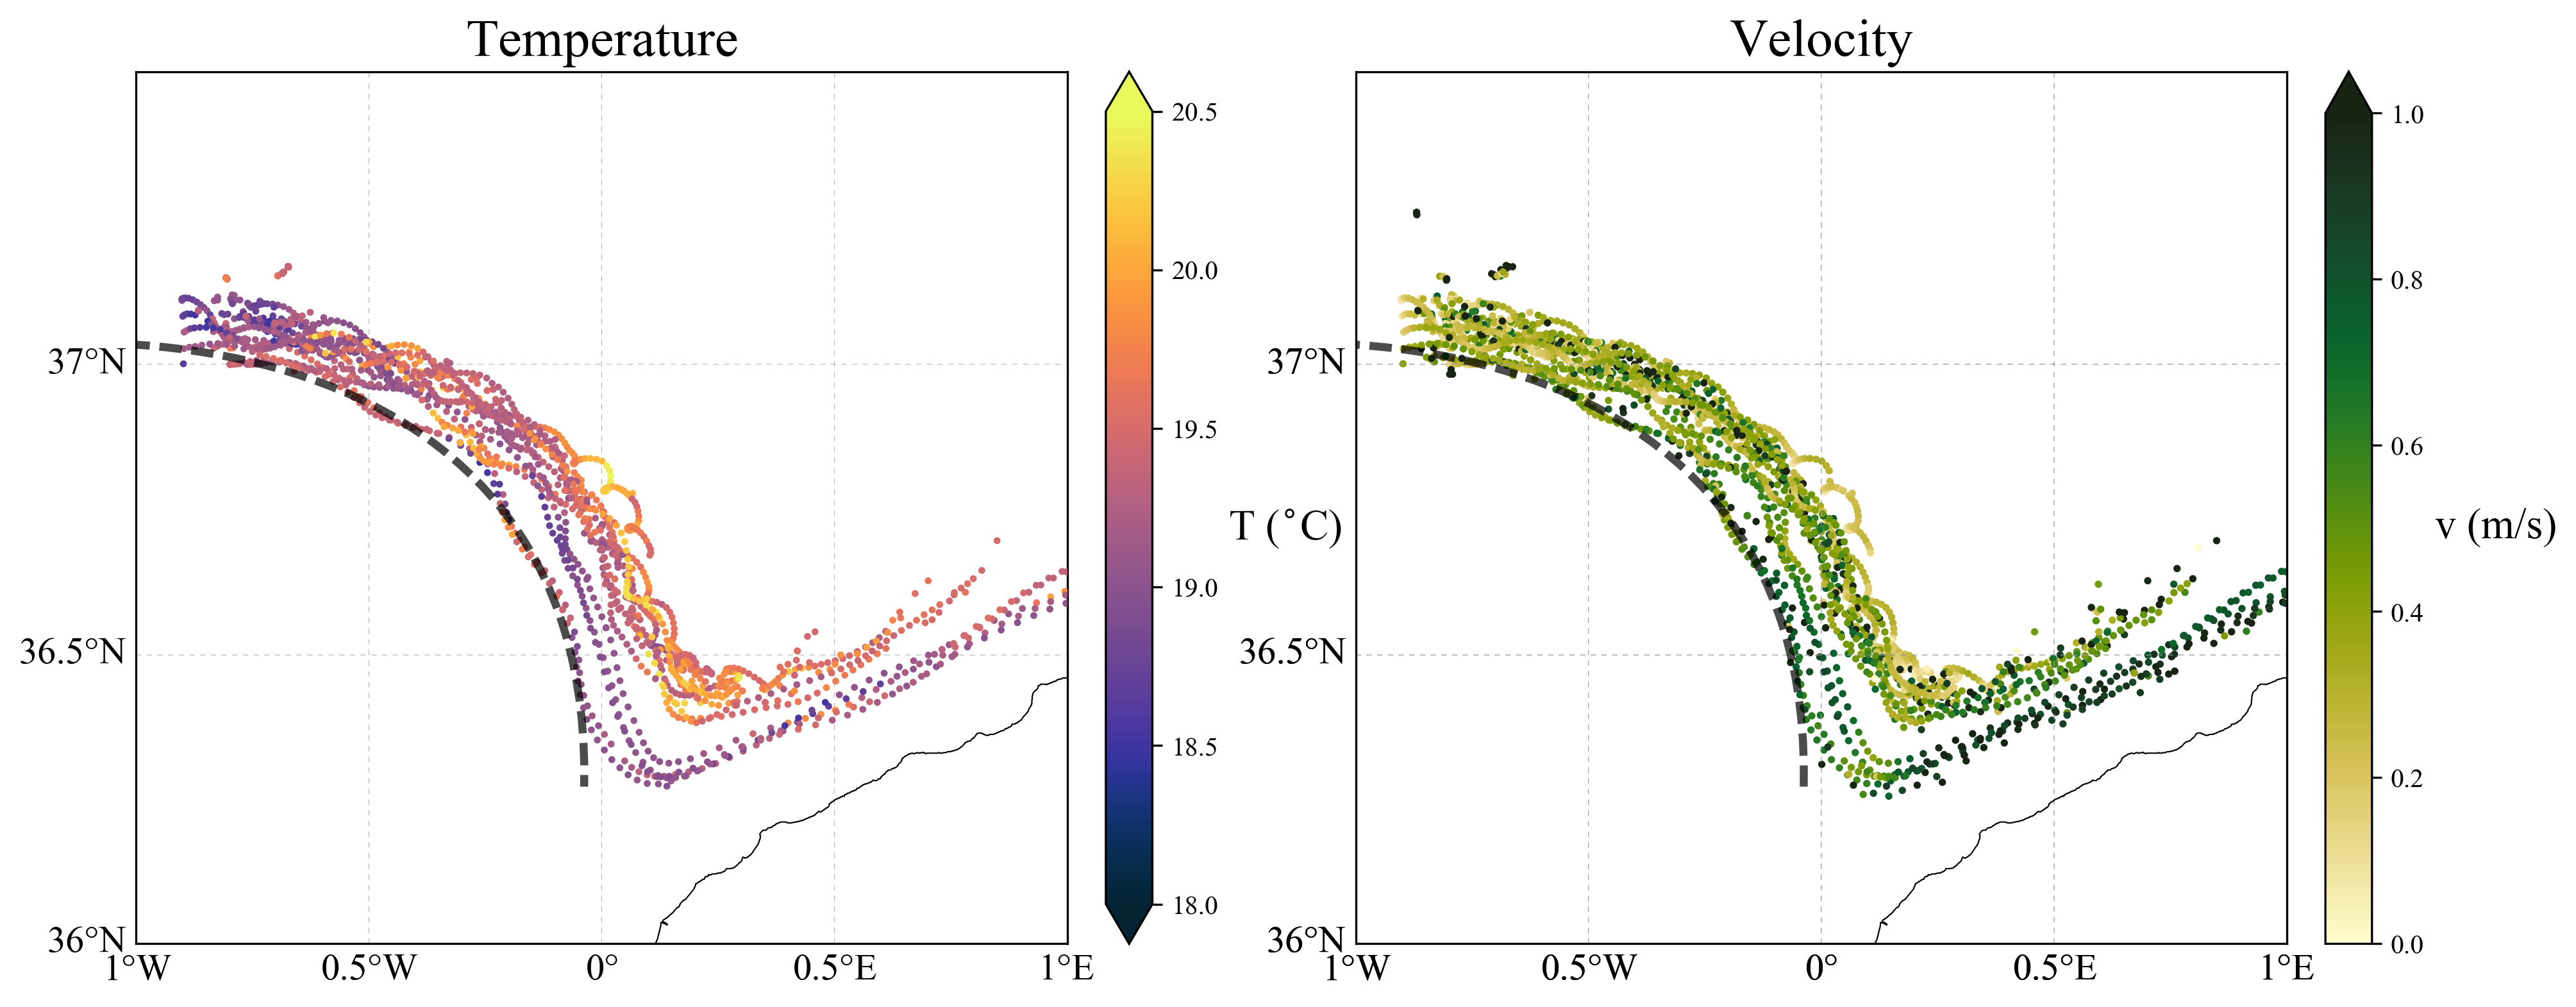
\includegraphics[width=.9\textwidth]{fig07cd.png}
\caption{Drifter temperature (left-hand side) and velocity in the area of study.\label{fig7:drifterszoom}}
\end{figure*}


\subsubsection{Profiling floats}

Three profiling floats were deployed in the same zone as the drifters, on May 25 (see Tab.~\ref{tab:argofloats}). Their configuration depends on the float type: the Arvor-C has higher temporal resolution (hours) and does not go much deeper than 400~m. The A3 and Provor-bio platforms are usually set to have cycle length between 1 and 5 days, with the bio reaching maximal depth on the order of 1000~m. The floats constitute an essential tool in order to monitor the mesoscale \citep{SANCHEZROMAN17}. The trajectories (Fig.~\ref{fig8:argofloats}) clearly show that profiles were acquired in the frontal area, before the floats were eventually captured by the Algerian Current. 

The Arvor-C trajectory closely follows the front position until a latitude of 36$\circ$30'N, accounting for 455 profiles in the vicinity of the front. This is probably due to its configuration: its high frequency temporal sampling makes it possible to spend more time in the near-surface layer and hence the float follows the front better than the 2 other float types. Its last profile was taken on June 14, 2014, at an approximative location of 36$\circ$15'N, 4$^{\circ}E$, then it drifted at the surface.

The 2 Arvor-type floats provided temperature and salinity profiles. In addition to T and S, the Provor-bio platform measured biochemical and optical properties: colored dissolved organic matter (CDOM), chlorophyll-a concentration, backscattering (650~nm), dissolved oxygen concentration and downwelling  irradiance (380, 410, 490~nm) and photosynthetically active radiation (PAR). The profiles were performed around local noon time and were used in combination with the glider measurements to study the deep chlorophyll maximum (DCM) across the front \citep{OLITA17}.

\begin{figure*}[h]
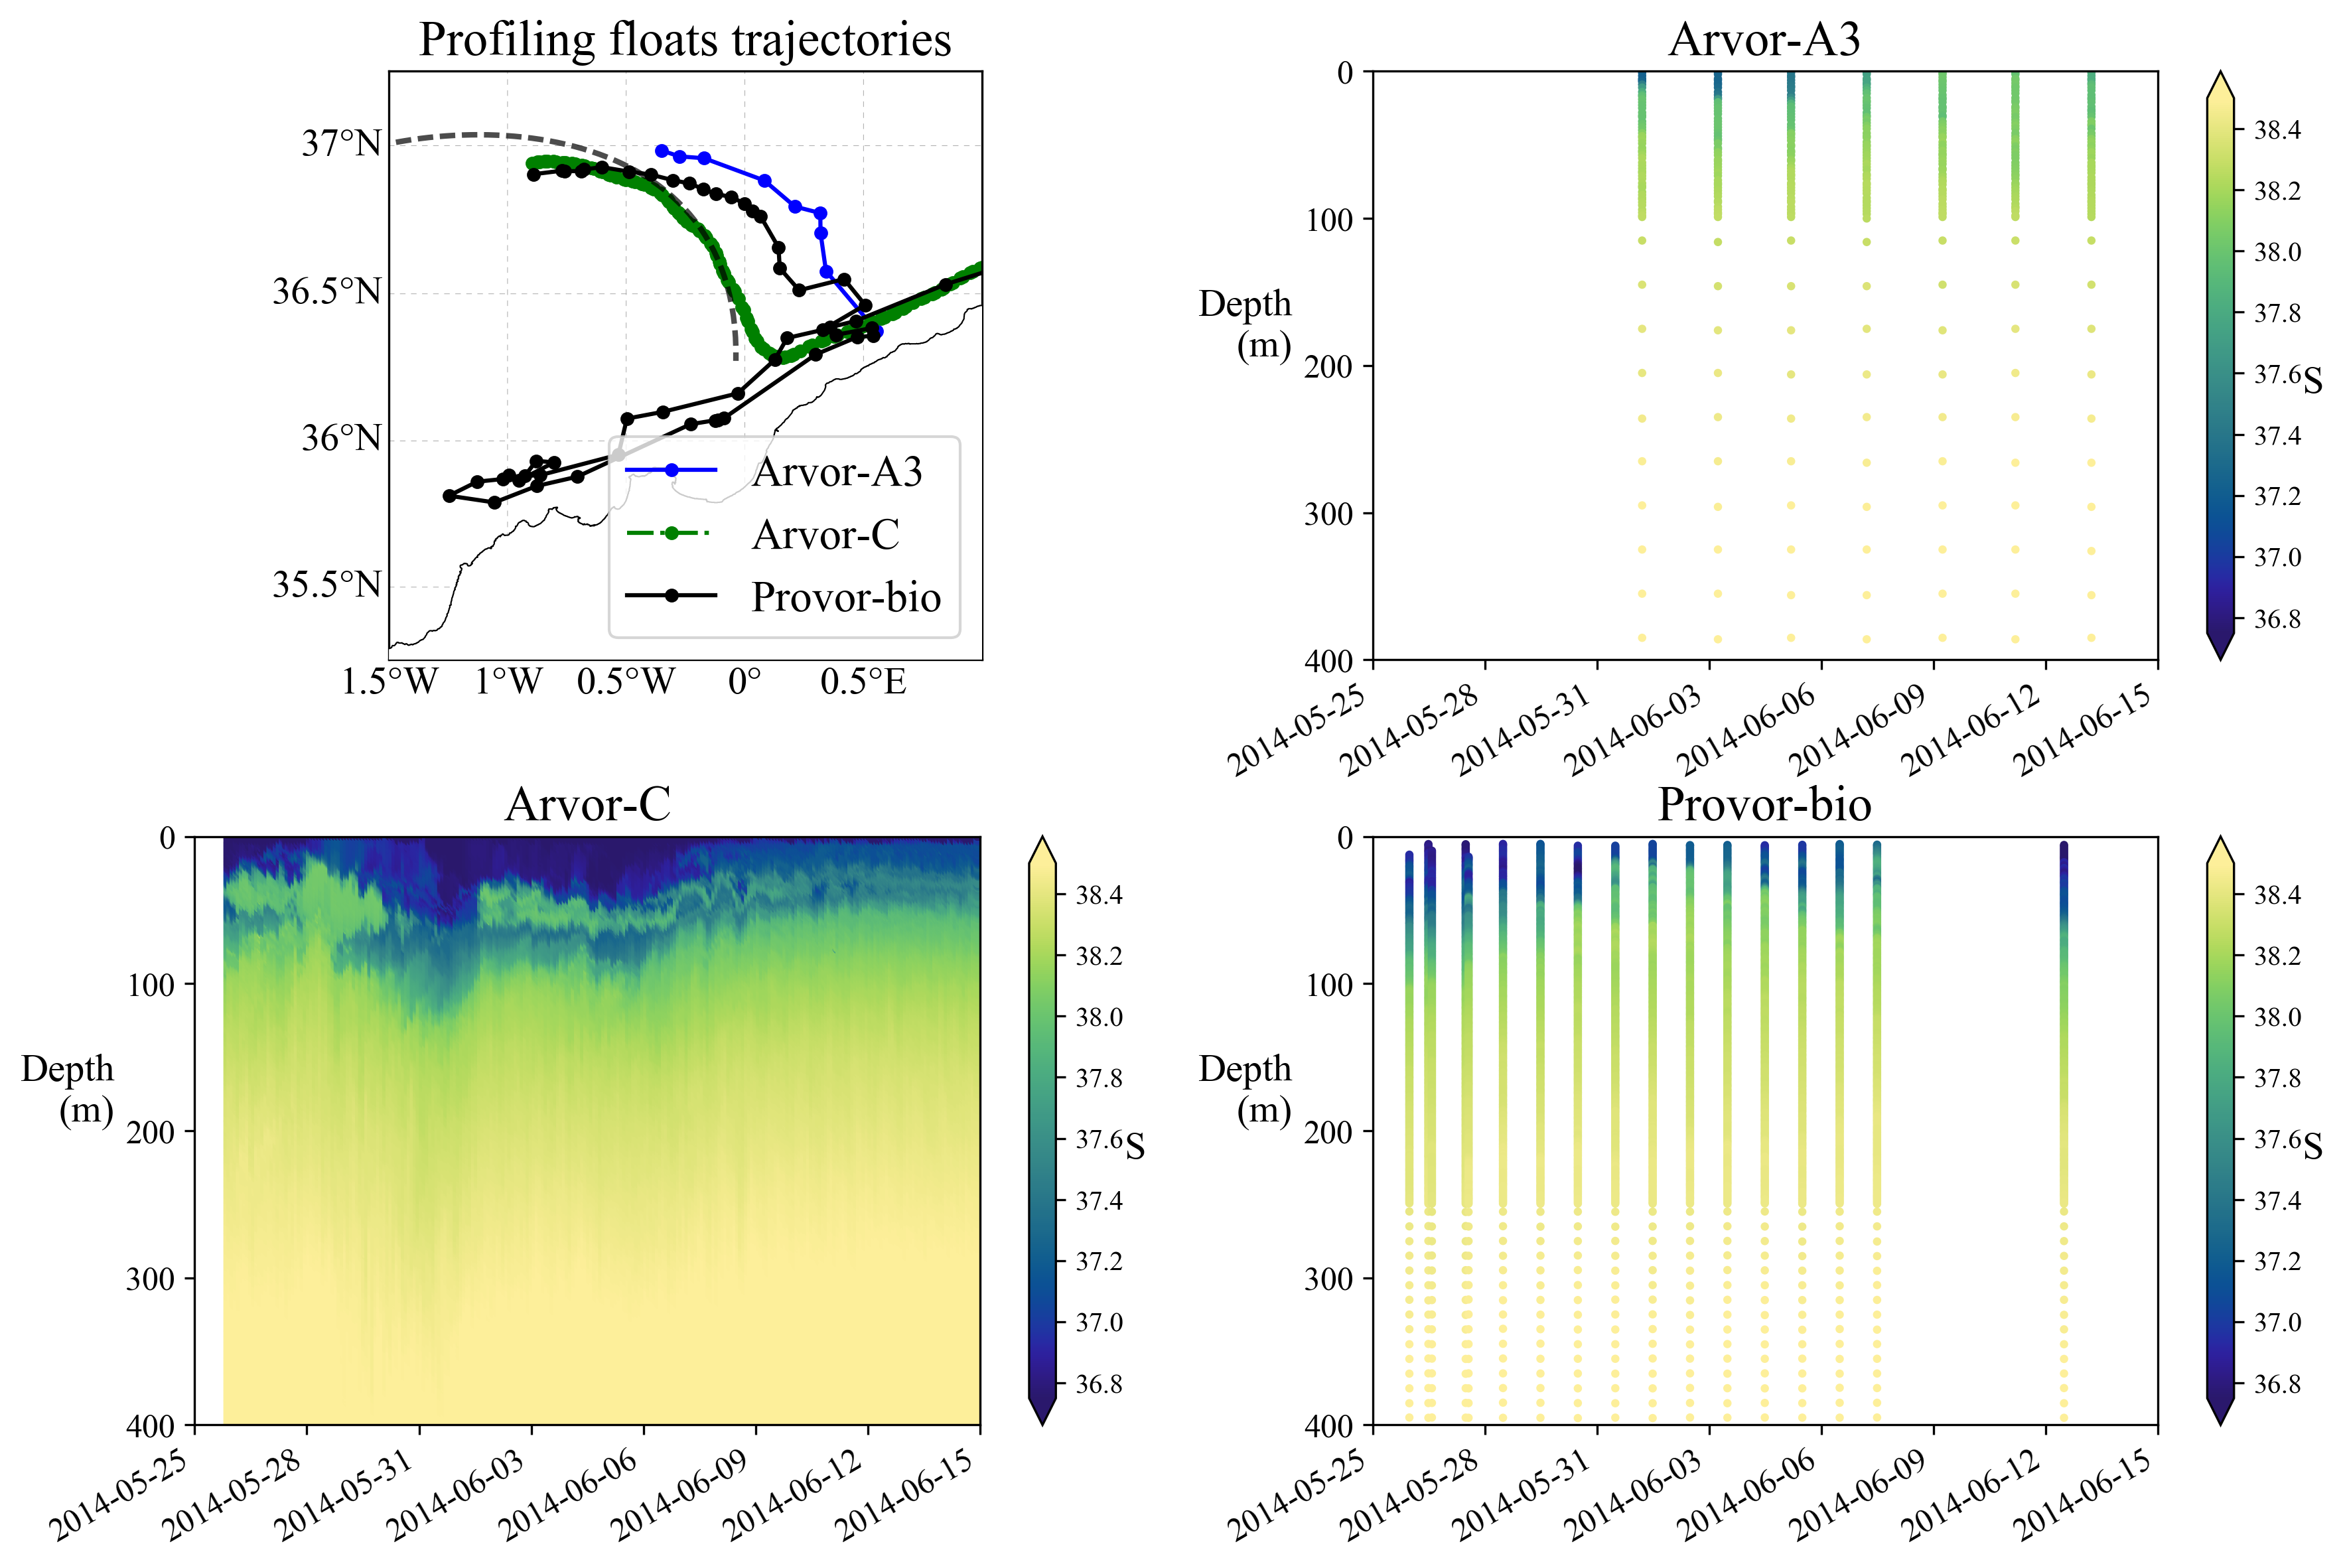
\includegraphics[width=.9\textwidth]{fig08a.png}
\caption{Profiling floats trajectories (top-left panel) and salinity from May 25 to June 15, 2014. \label{fig8:argofloats}}
\end{figure*}


\begin{table*}[htpb]
\caption{Characteristics of the profiling floats.\label{tab:argofloats}}
\begin{tabular}{lccllc}
\tophline
Platform 			& Initial time	& Final time	& Maximal depth (m)		& Period & Number of profiles \\
\middlehline
Arvor-A3			& 2014-05-25	& 2014-06-17	& 2000		& 1 day 	& 12 							\\ 
Arvor-C				& 2014-05-25	& 2014-06-17	& 400		& 1.5 hour	& 455				\\ 
Provor-bio			& 2014-05-25	& 2014-07-13	& 1000		& 1 day until June 7, then 5 days	& 71	\\ 
\bottomhline
\end{tabular}
\end{table*}

\subsubsection{Current profiler\label{sec:adcp}}

The Vessel Mounted-Acoustic Doppler Current Meter Profiler (VM-ADCP) operating at 153 kHz acquired velocity profiles approximatively every 2 minutes during nighttime (22:00--6:00 UTC) at a speed of 10 knots and during the CTD surveys (see Fig.~\ref{fig3:CTD}). The measurement accuracy is on the order of 0.01~m/s. The measurements were vertically averaged over 8~m depth bins.

The velocities exhibit a dominant eastward current with speed locally larger than 1~m/s and that signal is clearly visible in the first 100~m of the water column. The velocity field is illustrated in Fig.~\ref{fig9a:adcp} where each velocity vector is shown as a bar with a color depending on the intensity. The vertical structure is also displayed along with the front position.

\begin{figure*}[h]
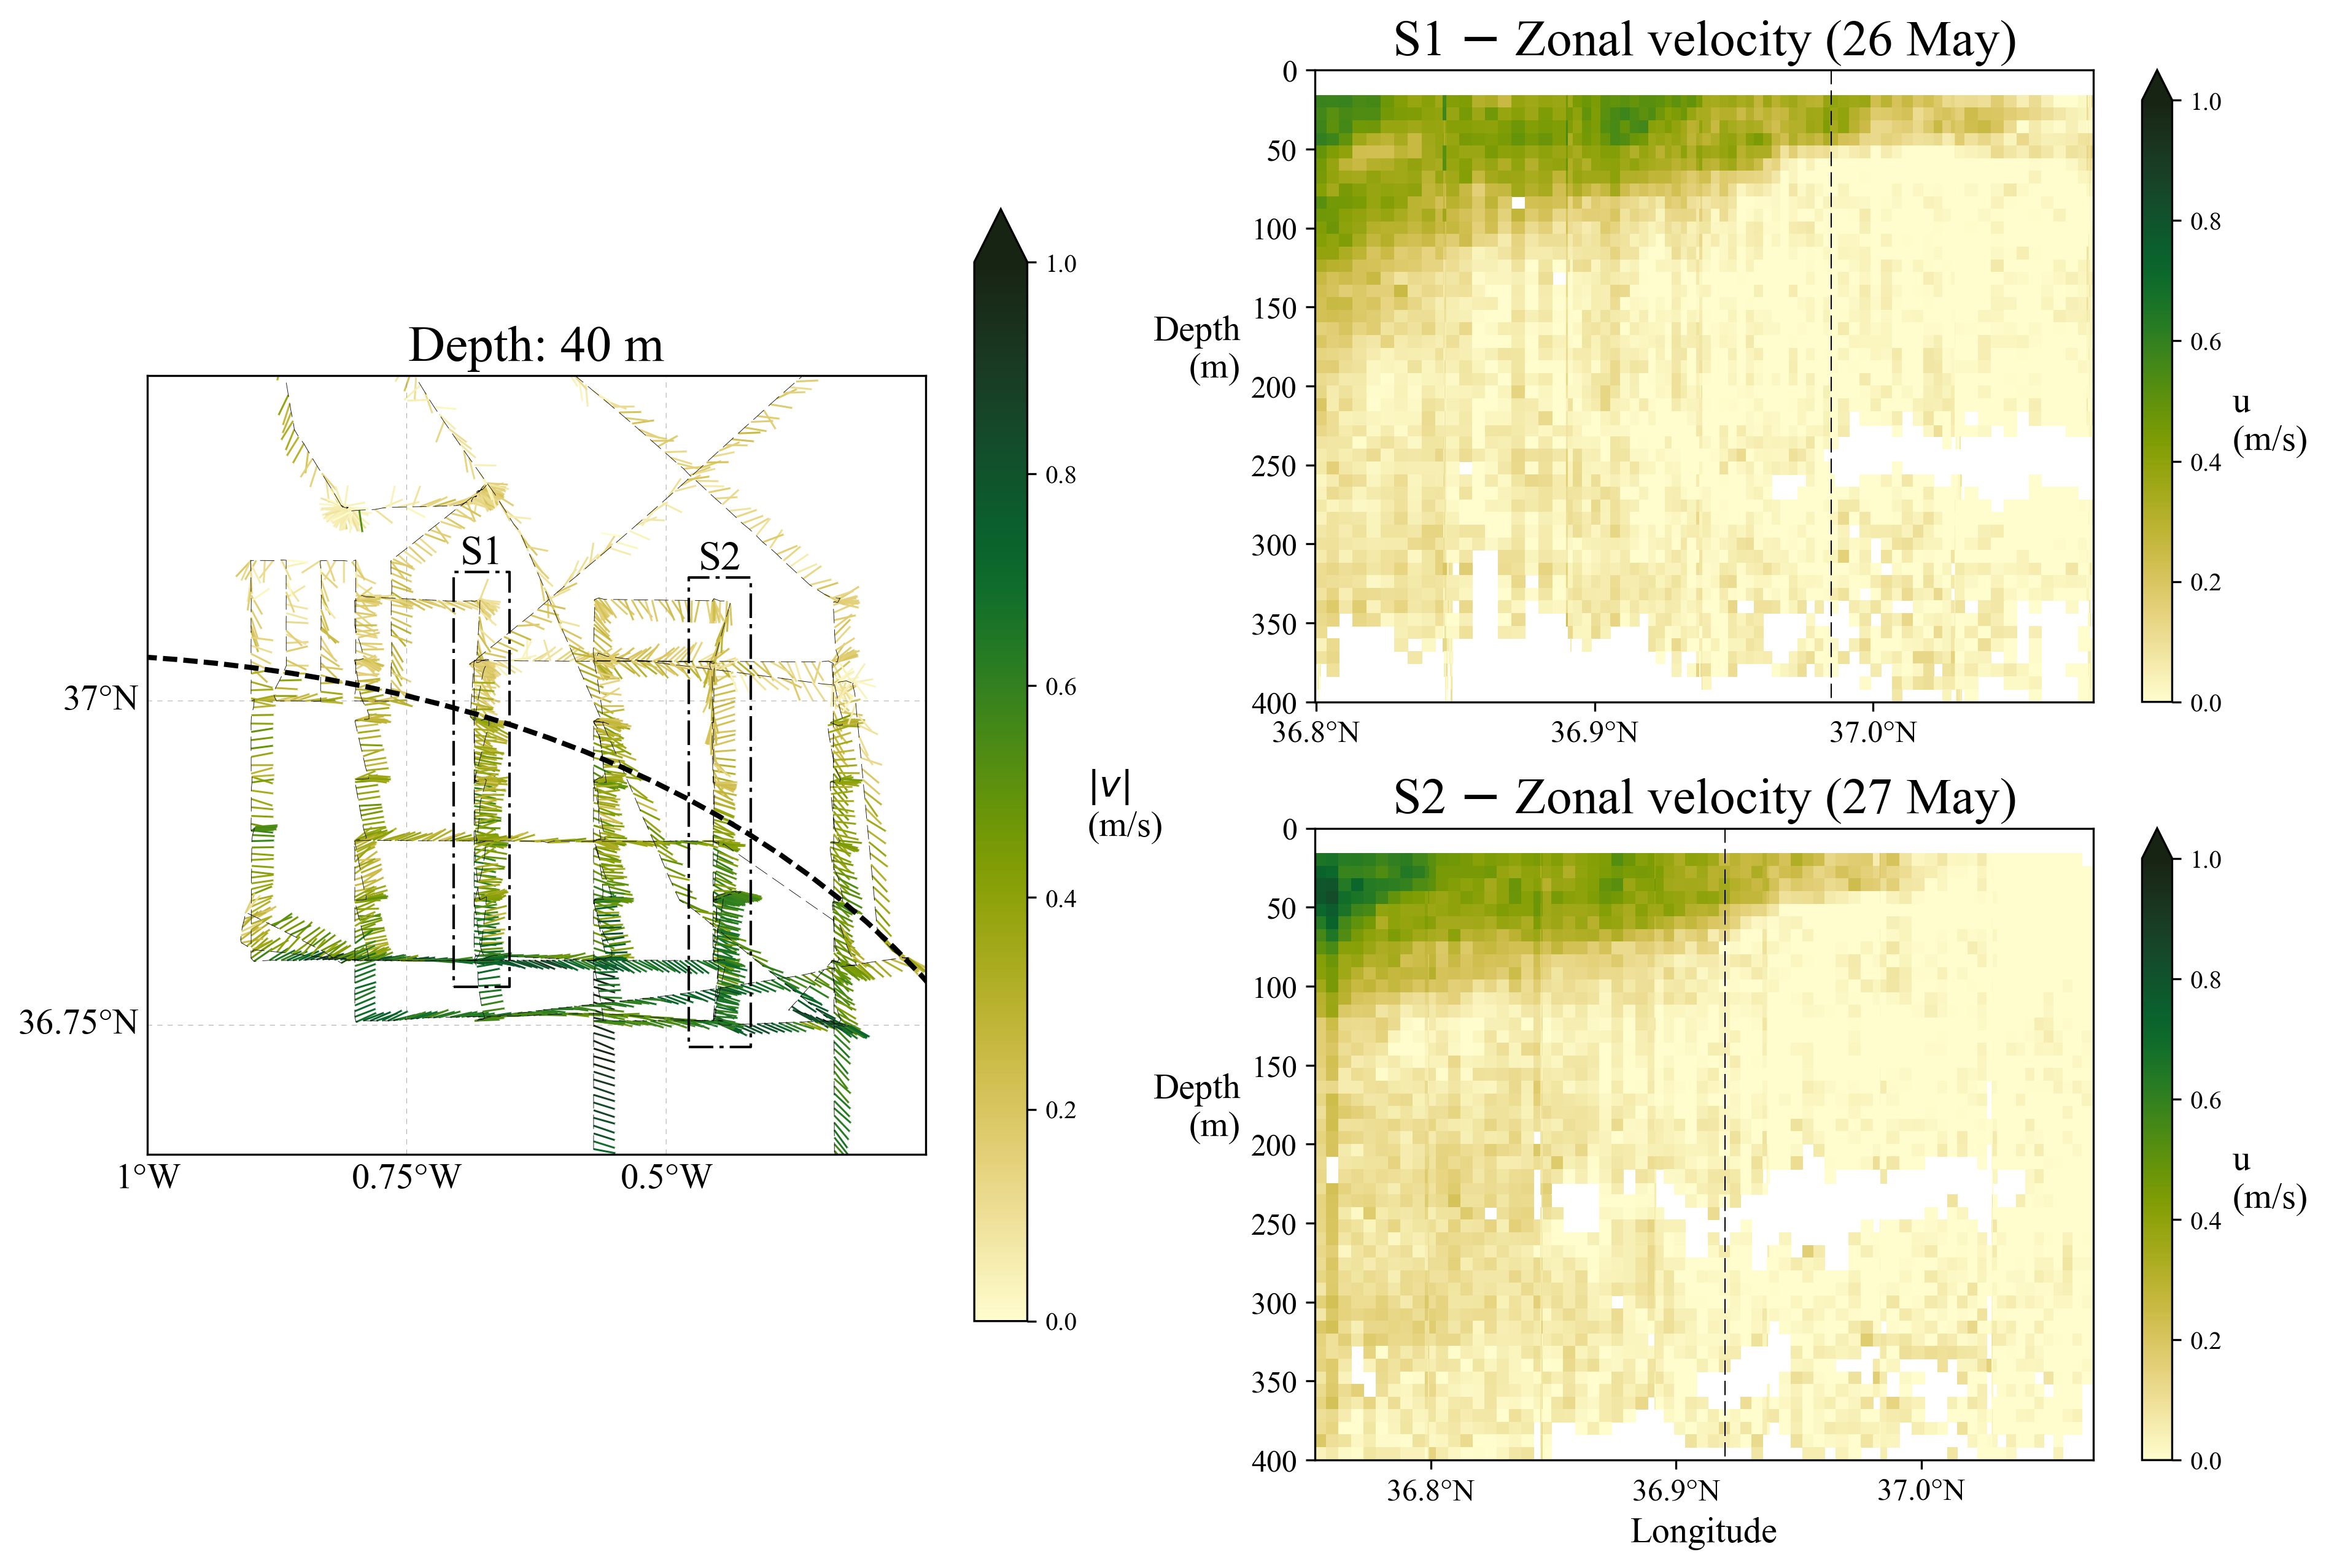
\includegraphics[width=.95\textwidth]{fig09a.png}
\caption{Velocity field obtained with the ADCP at a 40~m depth (left panel) and sections of zonal velocity on May 26 (S1) and 27 (S2). The locations of the sections are indicated by dashed rectangles on the map. Only data with a quality flag equal to 1 (good data) are represented\label{fig9a:adcp}}
\end{figure*}

This type of current measurements requires a careful processing in order to get meaningful velocities from the raw signal, hence it is relevant to have a quality flag (QF) assigned to each measurement. The quality checks applied for this platform were adapted from the quality control (QC hereinafter) relative to the ADCP mounted on a mooring.

Figure~\ref{fig9b:adcpQC} shows the QF during the whole mission. The 3 main periods during which the ADCP was turned off are shown as grey areas. In addition, no measurements are available in the first meters of the water column, due to the position of the ADCP on the ship.

\begin{figure}[h]
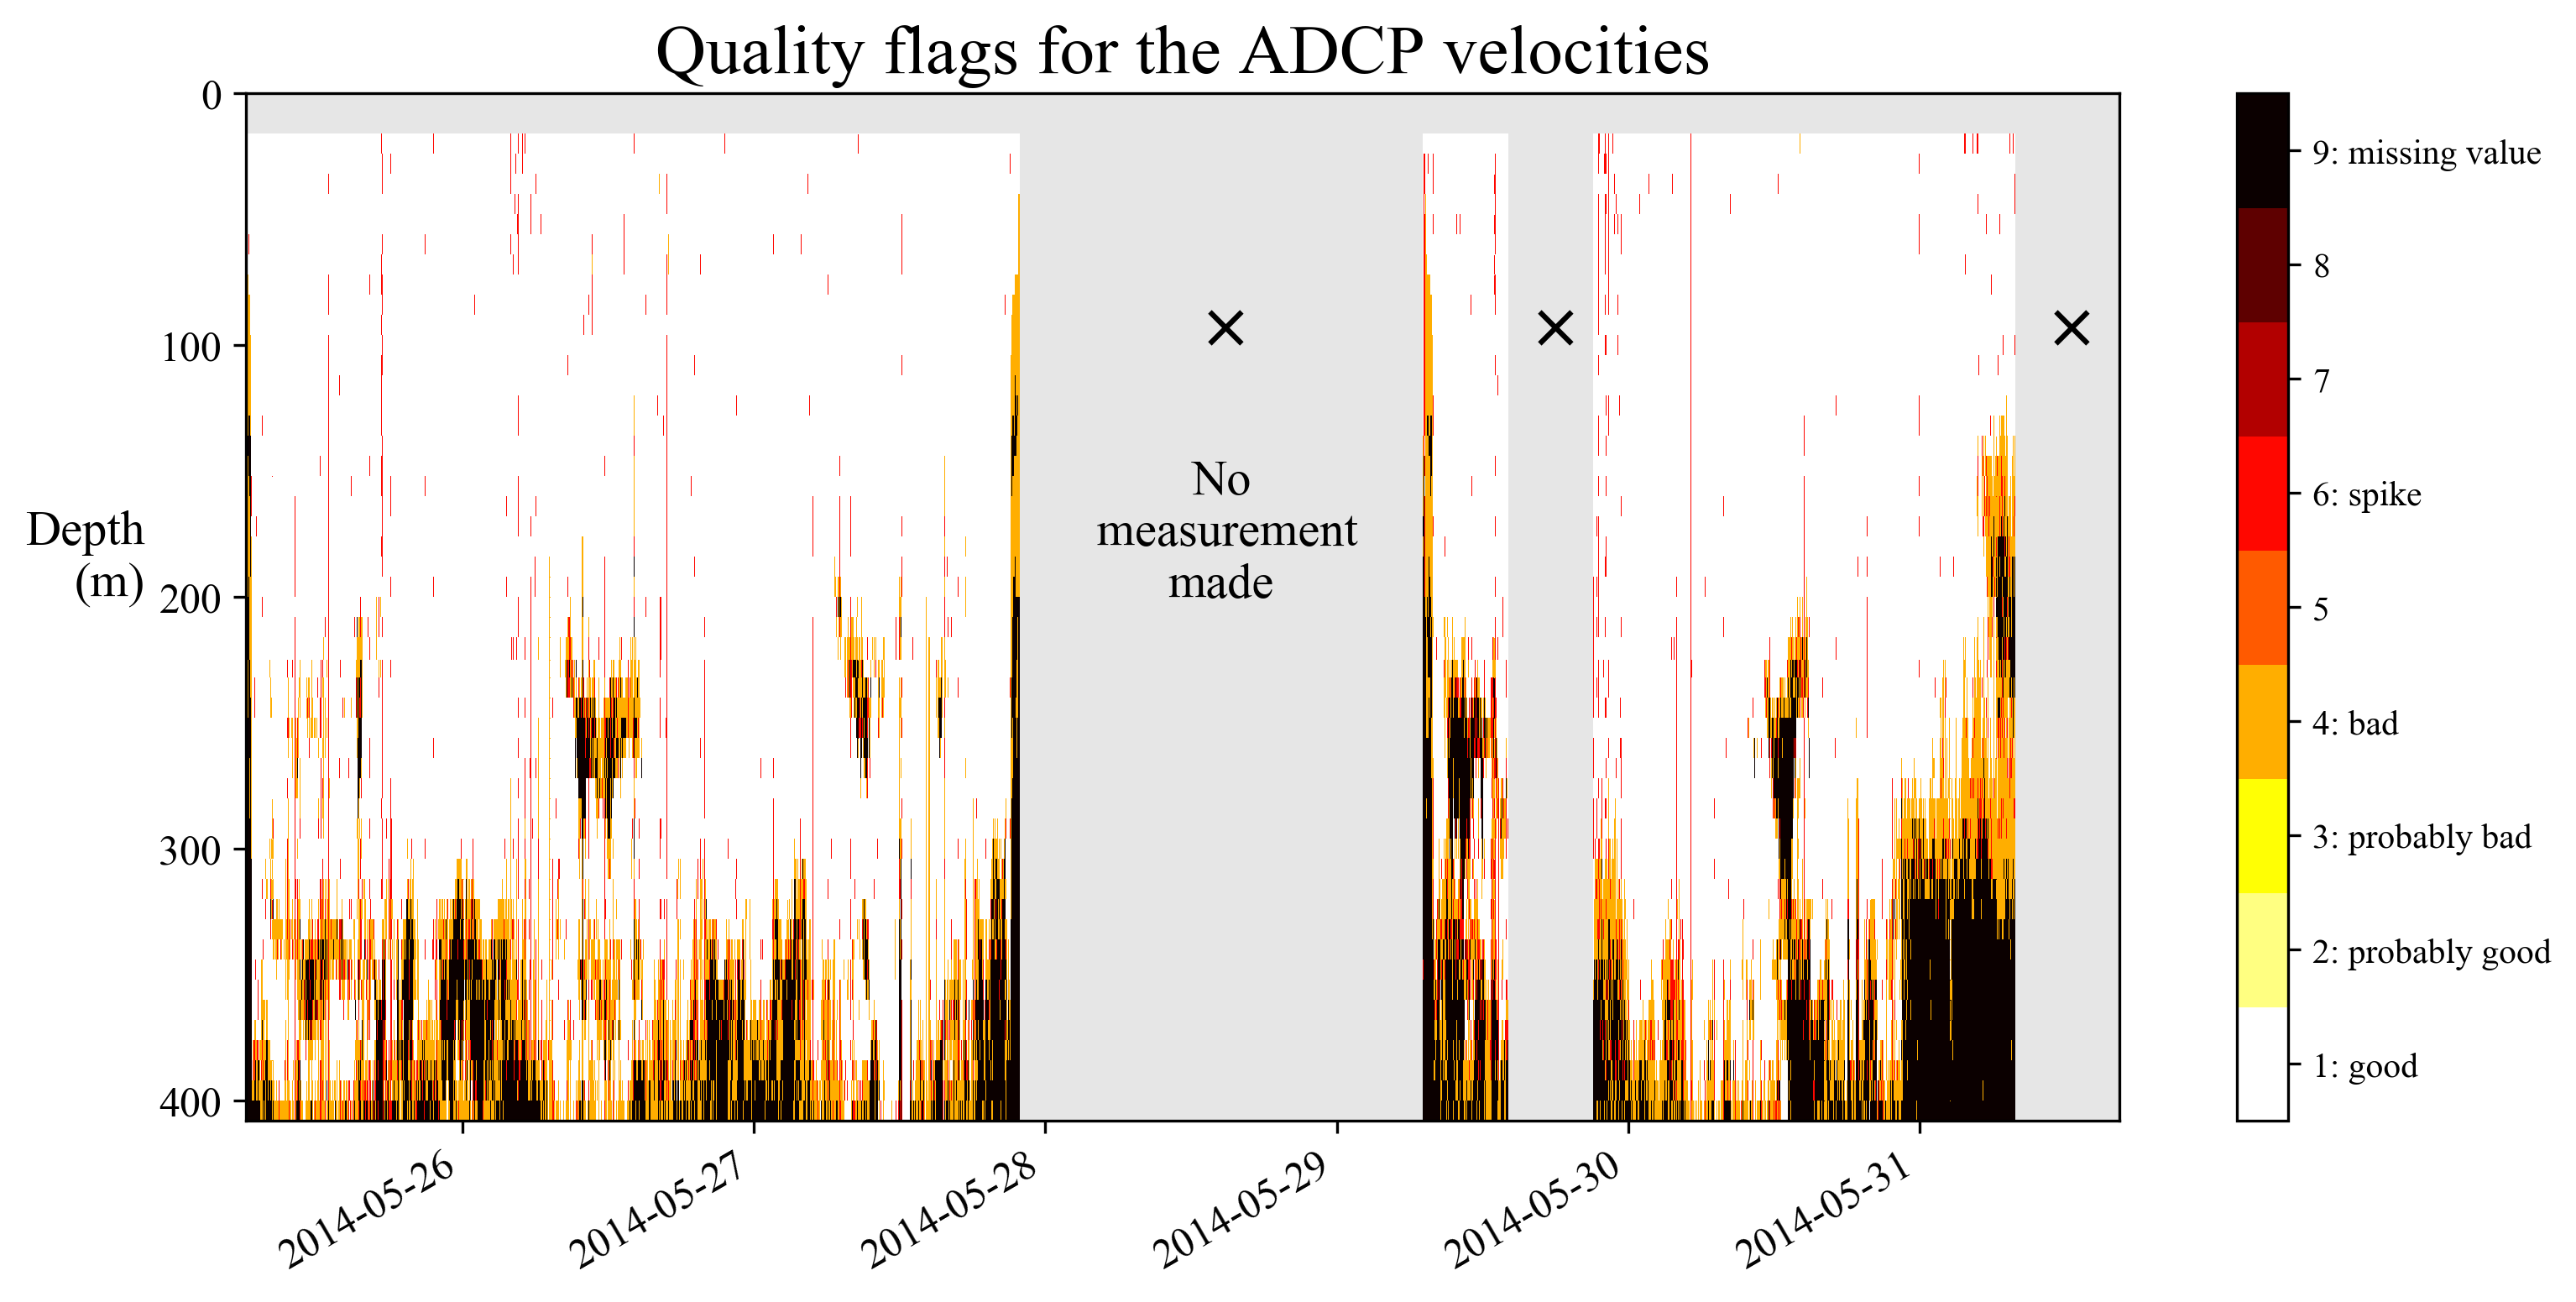
\includegraphics[width=.475\textwidth]{fig09b.png}
\caption{Quality flags for the velocity measurements.\label{fig9b:adcpQC}}
\end{figure}

Overall the quality of the data tends to deteriorate when the depth increases, as reflected by the bad and missing values. In the first 200~m, about 95\% of the measurements are considered as good. Below 200~m, the ratio drops to 57\% with more than 21\% of missing values. Note that the flags 5, 7 and 8 were not used in this case but kept in the plot.

\section{Description of the database\label{sec:database}}

The AlborEx mission generated a large amount of data in a region sparsely sampled in the past. The synergy between lower-resolution (CTD, drifters, floats) and high-resolution data (ADCP, gliders) makes this dataset unique for the study of submesoscale processes in the Mediterranean Sea. Moreover its multidisciplinary nature makes it suitable to study the interactions between the physical conditions and the biogeochemical variables.

\subsection{File format and organisation}

The original data files (i.e. obtained directly from the sensors and with a format depending on the manufacturer) are converted to Network Common Data Form (netCDF, \doi{(http://doi.org/10.5065/D6H70CW6}, last accessed on August 3, 2018), an Open Geospatial Consortium (OGC) standard widely adopted in atmospheric and oceanic sciences. Each file contains the measurements acquired by the sensors as well the metadata (mission name, principal investigator, \ldots). The structure of the files follows the Climate and Forecast (CF) conventions \citep{DOMENICO13} and are based on the model of OceanSITES \citep{SEND2010}. 

\subsection{File naming}
In order to keep the file names consistent with the original database, it is decided to keep the same file names as those assigned by SOCIB Data Center. Let us decompose one file name into its different parts: 
\texttt{dep0007\_socib-rv\_scb-sbe9002\_L1\_2014-05-25.nc}
\begin{description}
\item[\tt dep0007] indicates the number of the deployment, where deployment is the equivalent to the start of a mission or survey with a given platform. The deployment ends when the mission is over or if the platform stops acquiring data.
\item[\tt socib-rv] is the code for the platform, in this case the SOCIB coastal research vessel.
\item[\tt scb-sbe9002] is the instrument identifier, here the CTD SeaBird 9Plus. Note that the instrument is described in the metadata of the netCDF file.
\item[\tt L1] is the processing level (see Sec.~\ref{sec:processing}).
\item[\tt 2014-05-25] is the deployment date (year-month-day).
\end{description}
Now the general naming is defined, Tab.~\ref{tab:filenales} list below the different files made available in the dataset.
\begin{table*}[h]
\caption{Platform corresponding to the different files.\label{tab:filenales}}
\begin{tabular}{ll}
\tophline
File name				& Platform 															\\
\middlehline
\verb#dep0023_socib-rv_scb-rdi001_L1_2014-05.nc#					& ADCP								\\
\verb#dep0007_socib-rv_scb-sbe9002_L1_2014-05-25.nc#				& CTD 								\\
\verb#dep0001_drifter-svp***_scb-svp***_L1_2014-05-25.nc#			& SVP drifers ($\times$ 25)		\\
\verb#dep0005_icoast00_ime-slcost000_L1_2014-05-25_data_dt.nc#	& Coastal glider 					\\
\verb#dep0012_ideep00_ime-sldeep000_L1_2014-05-25_data_dt.nc#		& Deep glider 	 					\\
\verb#dep0001_profiler-drifter-arvora3001_ogs-arvora3001_L1_2014-05-25.nc#	& Arvor-A3 float		\\
\verb#dep0001_profiler-drifter-arvorc_socib_arvorc_L0_2014-05-25.nc# 			& Arvor-C float			\\
\verb#dep0001_profiler-drifter-provbioll001_ogs-provbioll001_L1_2014-05-25.nc# & Provor-Bio float	\\
\verb#dep0015_socib-rv_scb-met009_L1_2014-05-25.nc#				& Weather onboard  R/V 				\\
\verb#dep0015_socib-rv_scb-pos001_L1_2014-05-25.nc#				& Navigation data from R/V 		\\
\verb#dep0015_socib-rv_scb-tsl001_L1_2014-05-25.nc#				& Thermosalinograph					\\
\verb#dep0015_socib-rv_scb-tsl001_L1_2014-05-25_HR.nc#			& Thermosalinograph (high-res.)	\\
\bottomhline
\end{tabular}
\belowtable{\texttt{***} in the file names stands for 3 digits.} 
\end{table*}

\subsection{Data processing\label{sec:processing}}

For each of the platform described in Sec.~\ref{sec:mission}, different processing are performed with the objective to turn raw data into quality-controlled, standardised data directly usable by scientists and experts. Specific conventions for data managed by SOCIB are explained below.

\subsubsection{Processing levels}

All the data provided by SOCIB are available in different so-called processing levels, ranging from 0 (raw data) to 2 (gridded data). The files are organized by \textit{deployments}, where a deployment is defined as an event initiated when an instrument is put at sea and finished once the instrument is recovered from sea. Table~\ref{tab:deployment} summarizes the deployments performed during the experiment and the available processing levels.

\begin{description}
\item[Level 0 (L0)]: this is the level closest to the original measurements, as it contains exactly the same data as the raw files provided by the instruments, but in a single file.
\item[Level 1 (L1)]: in this level, additional variables are derived from the existing ones (e.g., salinity, potential temperature). The attributes corresponding to each variable are stored in the netCDF file, with details of any modifications. Unit conversion are also applied if necessary.
\item[Level 2 (L2)]: this level consists of regular, homogeneous and instantaneous profiles obtained by interpolating the L1 data. It is only provided for gliders, mostly for visualization and post-processing purposes: specific tools designed to read and display profiler data can then be used the same way for gliders.
\end{description}
The glider data require a specific processing to ingest and convert the raw data files produced by the coastal and deep units. This is done within a toolbox designed for this purpose and extensively described in \citet{TROUPIN16}, the capabilities of which includes metadata aggregation, data download, advanced data processing and the generation of data products and figures. Of particular interest is the application of a thermal-lag correction for un-pumped Sea-Bird CTD sensors installed on Slocum gliders \citep{GARAU11}, which improves the quality of the glider data.

\begin{table*}[htpb]
\caption{Characteristics of the instrument deployments in AlborEx.\label{tab:deployment}}
\begin{tabular}{lcrrccc}
\tophline
Instruments 		& Number of deployments & Initial time	& Final time			& \multicolumn{3}{c}{Processing levels} \\
					& 						& 				& 						& L0 			& L1 		& L2 \\
\middlehline
Weather station on board R/V	& 1			& 2014-05-25	& 2014-05-02			& \checkmark	& \checkmark &  \\ 
ADCP on board R/V	& 1						& 2014-05-25	& 2014-05-02			& \checkmark	& \checkmark &  \\ 
CTD					& 1 (66 stations)		& 2014-05-25	& 2014-05-02			& \checkmark	& \checkmark &  \\ 
Gliders 			& 2						& 2014-05-25	& 2014-05-30 			& \checkmark 	& \checkmark & \checkmark \\
Surface drifters	& 25					& 2014-05-25	& beyond the experiment & \checkmark 	& \checkmark &  \\
Profiling floats	& 3						& 2014-05-25	& beyond the experiment & \checkmark 	& \checkmark &  \\
\bottomhline
\end{tabular}
\belowtable{} % Table Footnotes
\end{table*}

\subsubsection{Quality control}

Automated data QC is part of the processing routine of SOCIB Data Center: most of the datasets provided with this paper come with a set of flags that reflect the quality of the measurements, based on different tests regarded the range of measurements, the presence of spike, the displacement of the platform and the correctness of the metadata. 

\begin{description}
\item[Drifters:] checks are performed to remove bad positions (i.e. on land) and spikes in the trajectory. For the SVP drifters, the method developed by \citep{RIO12} is used to improve the accuracy of the drogue presence from wind slippage \citep{MENNA18}.
\item[Profiling floats:] standard tests are performed to check the time and the position accuracy. Variable ranges are checked at each depth.
\end{description}

For some platforms, the automated QC are not implemented yet:
\begin{description}
\item[Gliders:] a set of quality checks have been added to the glider toolbox \citep[][and available at \url{https://github.com/socib/glider_toolbox}]{TROUPIN16} and are in testing phase at the time of the writing. The QC included tests on $NaN$ values, impossible date or location, valid ranges (depending on depth) for the variables, spikes, gradients and flat lines (constant value over a large range of depths) in profiles. The later check proved useful for conductivity (and hence density and salinity). This new QC step will then be included to the general procedure and new netCDF files will be produced and made available as a new version of the present dataset.
\item[CTD profiles:] the situation is similar to the gliders: new tests have been recently added to the processing chain at SOCIB, hence the AlborEx CTD profiles will have to be reprocessed in order to assign the quality flags to the measurements. These tests are essentially based on the range of measured values depending on each variable and the presence of strong vertical variations spike within a profile.
\end{description}

As the new files will not be available before a full reprocessing of all the historical missions, we decided to provide the data files in their current state. A new version will be uploaded as soon as the processing has been performed.


\conclusions[Conclusions and perspectives]

The AlborEx observations acquired in May 2014 constitutes a unique observational data set that captured mesoscale and submesocale features in a particularly energetic frontal zone in the western Mediterranean Sea. The potential uses of the dataset can be separated in different topics:
\begin{itemize}
\item Hydrodynamics model validation: but the timing and location of small-scale features 
\item High-resolution remote-sensing data validation: high quality in situ measurements of the sea surface are essential for the validation of operational product such SST or Ocean Color. 
\item Study of mechanisms: the Mediterranean Sea is often referred to as a laboratory for oceanography and in particular the Alboran Sea is the stage of intense processes of mixing, subduction and instabilities.
\item Assessment of mechanisms responsible for intense vertical motions.
\end{itemize} 

The version of the dataset described in the present paper contains files that have been processed and standardised so that they are directly usable by scientists without having to perform unit or format conversions from the manufacturer raw data files.

Updates will be performed when new versions of the files or new files are made available.

\codedataavailability{
Following SOCIB general policy, the data are made available as netCDF files through the SOCIB Thematic Real-time Environmental Distributed Data Services (THREDDS) Data Server, a standard way to distribute metadata and data using a variety of remote data access protocols such as OPeNDAP (\url{https://www.opendap.org}), Web Map Service (WMS) or direct HTTP access. 
In addition, the whole AlborEx dataset has been uploaded Zenodo (\url{https://zenodo.org/}, last accessed in August 3, 2018), a research platform designed to store any type of research outputs (papers, code, datasets) and assigns a Digital Object Identifier (DOI) to make them easily and uniquely citable.
The most recent version of the dataset is accessible from \url{http://doi.org/10.5281/zenodo.1328238}.

Upgrades will be performed periodically with the implementation of fresh or better QCs on sensors such as the ADCP, CTD or gliders. The new releases will be available using the same Zenodo identifier, but with be assigned a different version number, each version having its own DOI. Files not available at the time of the writing will also be appended to the original database. 

Concerning the improvement of the quality control, it is worth mentioning the new tests that will be implemented in the SOCIB Glider Toolbox \citep{TROUPIN16}.

The checks performed on the ADCP velocities involve a set of parameters that can also be fine-tuned to improve the relevance of the quality flags. Nevertheless, noticeable changes are not expected with respect to the quality flags displayed in Fig.~\ref{fig9b:adcpQC}.

Finally, the quality of the CTD and the glider profiles can be improved by using the salinity measurements of water samples collected during the mission. This type of correction might not be essential for the study of mesoscale processes but is crucial when one is focused on long-term studies and when a drift can be observed in the salinity measurements.

A set of programs in Python to read the files and represent their content as in the figures presented through the paper are available at \url{https://github.com/ctroupin/AlborEX-Data}. The programs are written in the form of documented Jupyter notebooks, a web application that combines code fragment, equations, graphics and explanatory text (\url{http://jupyter.org/}, last accessed 14 August, 2018) so that they can be run step by step. The figures colormaps were produced using the \texttt{cmocean} module \citep{THYNG16}.
}
\authorcontribution{C.T. prepared the figures and the first version of the manuscript. A.P. and S.R. edited the manuscript. J.G.F. and M.A.R. lead the data management and the creation of a DOI in Datacite. C.M. implemented the processing of the ADCP data. G.N. helped with the processing of the drifters and profiling floats.}

\competinginterests{The authors declare that the research was conducted in the absence of any commercial or financial relationships that could be construed as a potential conflict of interest.}

\disclaimer{The authors do not accept any liability for the correctness and appropriate interpretation of the data or their suitability for any use.}

\begin{acknowledgements}
AlborEx was conducted in the framework of PERSEUS EU-funded project (Grant agreement no.~287600). Glider operations were partially funded by JERICO FP7 project. AP acknowledges support from the Spanish National Research Program (E-MOTION/CTM2012-31014 and PRE-SWOT/CTM2016-78607-P). SR and AP are also supported by the Copernicus Marine Environment Monitoring Service (CMEMS) MedSUB project. AO was supported by the Jerico-TNA program, through the FRIPP (FRontal Dynamics Influencing Primary Production) project. The profiling floats and some drifters were contributed by the Argo-Italy program. The proceedings of such an ambitious mission would not have been possible without the involvement of a numerous staff both at sea and on land: A.~Massanet, M.~Palmer, I.~Lizaran, C.~Castilla, P.~Balaguer, M.~Menna, K.~Sebastián, S.~Lora, and A.~Bussani .


\end{acknowledgements}

%% REFERENCES
\newpage

\bibliographystyle{copernicus}
\bibliography{AlborexData.bib}


\end{document}
